\documentclass[xcolor={usenames,dvipsnames}
    % ,handout
]{beamer}

%
% ugly hack referring to the slides folder. Works for me.
%
\makeatletter
\def\input@path{{../}}
\makeatother

% \usepackage[T1]{fontenc} % font encoding
% \usepackage{fontspec}
\usepackage{fontspec}


\makeatletter%
\@ifclassloaded{beamer}{%
  \usepackage{lmodern} %%% modern beamer style
  %%beamer style
  \usetheme{metropolis}
  \usefonttheme{professionalfonts}
  \setbeamercolor{background canvas}{bg=background}
  \setbeamercolor{frametitle}{bg=snow,fg=black}
  \setbeamercolor{title separator}{fg=snow}
  \setbeamercolor{alerted text}{fg=accent}

  \let\oldtitle\title
  \renewcommand{\title}[1]{\oldtitle{CMPUT391\\#1}}
  \author{Instructor: Denilson Barbosa}
  \date{\small University of Alberta}
  \institute{\today\vskip4em Slides by D. Barbosa, with suggested corrections and improvements by (in alphabetical order) C. Bins, D. Caminhas, K. Guhzva, Q. Lautischer, E. Macdonald, M. A. Nascimento, K. Newbury, M. Strobl, D. Sunderman, K. Wang, and K. Wong.}
  
  \titlegraphic{
\includegraphics[width=1.5cm]{../images/by-sa.png}~
  {\tiny This work is licensed under a Creative Commons Attribution 4.0 International License}}

  %%%% un-framed blocks
  \setbeamertemplate{blocks}[rounded][shadow=false]
}{}

\@ifpackageloaded{xcolor}{}{
  \usepackage{xcolor}
}
\makeatother

\setsansfont[BoldFont={Open Sans SemiBold}]{Open Sans}[Scale=0.9]
\setmonofont{Cousine}[Scale=0.875]
% \setmathtt{Cousine}[Scale=0.875]

%%%% highlighting text 
\usepackage{xspace}
\def\highlight#1{\colorbox{accent}{\textcolor{white}{#1}}\xspace}

\def\blue#1{\textcolor{blue}{#1}}

%
%
%
\usepackage{parskip}

\usepackage{subcaption} % needed for subfigures

\usepackage{wrapfig} % for figures "to the side of the text"

\usepackage{anyfontsize} % for egregious warnings

%
% Fonts
%
% \usepackage{amsmath}
% \usepackage{mathspec}
% \setmathtt[Scale=0.875]{Cousine}

%
% various packages for tables and colored tables
%
\usepackage{xcolor,colortbl}
\usepackage{tcolorbox}

\definecolor{accent}{RGB}{225,68,85}
\definecolor{highlight}{RGB}{170,68,153}
\definecolor{background}{rgb}{253,252,252}

\definecolor{sqlColor}{RGB}{119,119,17}

\definecolor{Cfunction}{RGB}{51,51,153}

\definecolor{stringColor}{RGB}{51,51,153}
\definecolor{datatypeColor}{RGB}{170,68,153}
\definecolor{functionColor}{RGB}{51,134,116}

\definecolor{exampleColor}{RGB}{51,34,136}
\definecolor{commentColor}{RGB}{112,68,225}

\definecolor{fern}{RGB}{80,118,66}

\definecolor{snow}{RGB}{240,240,230}
\definecolor{Gray}{gray}{0.85}

\definecolor{tupleBoxColor}{gray}{0.85}

\definecolor{Maroon}{RGB}{139,0,0}

%
% coloring of SQL code
%
\def\ColorSymbol#1{\textcolor{functionColor}{#1}}

%
% hihglight box
%
\usepackage{xspace}
\def\highlight#1{\colorbox{accent}{\textcolor{white}{#1}}\xspace}

%
% Tables
%
\usepackage{multirow}
\usepackage{multicol}

%
% CODE LISTINGS
%
\usepackage{listings}

%
% catch-all style meant to provide a clean and "empty" style
% from which all others build upon
%
\lstdefinestyle{cmput391}{
  style=,
  frame=no,
  tabsize=2,
  numbers=none,
  showstringspaces=false,
  numberstyle=\footnotesize,
  basicstyle=\ttfamily\footnotesize\color{black},
  numbersep=4pt,
  keywords=[1]{},
  keywords=[2]{},
  keywords=[3]{sh_lock,xl_lock,unlock,read,write,commit,abort},
  keywordstyle=[1]\ttfamily\bfseries\footnotesize,
  keywordstyle=[2]\ttfamily\footnotesize,
  keywordstyle=[3]\ttfamily\footnotesize\color{Maroon},
  emph=[1]{},
  emph=[2]{},
  emph=[3]{},
  emphstyle=[1]\ttfamily\footnotesize,
  emphstyle=[2]\ttfamily\footnotesize,
  emphstyle=[3]\ttfamily\footnotesize,
  commentstyle=\ttfamily\itshape\color{commentColor},
  stringstyle=\ttfamily\color{stringColor},
  moredelim=**[l][\itshape\color{commentColor}]{--},
  moredelim=**[is][\color{highlight}]{-|}{|-},
  moredelim=[is][\bfseries\color{highlight}]{-:}{:-},
  morestring=[s][\color{stringColor}]{"}{"},
  morecomment=[l]{--}
}

\lstdefinelanguage{DTD}{
  style=cmput391,
  morekeywords=[1]{DOCTYPE,ELEMENT,ATTLIST},
  keywordstyle=[1]\color{accent},
  literate = {\#PCDATA}{{\textcolor{Cfunction}{\#PCDATA}}}7
             {\#IMPLIED}{{\textcolor{Cfunction}{\#IMPLIED}}}8
}

\lstdefinelanguage{XPath}{
  style=cmput391,
  morekeywords={xs,integer,current,date,distinct,values,avg,text,id,count,position,and,or,not,boolean,number,sum,floor,ceiling,round,doc,eq,ne,gt,lt,ge,le},
  keywordstyle=\color{red},
  literate = {last(}{{\textcolor{functionColor}{last}(}}5 {@<}{{<}}1  
}

\lstdefinestyle{XQuery}{
  style=cmput391,
  keywords=[1]{if,then,else,and,or,some,every,satisfies,for,in,let,where,group,order,by,return,ascending},
  keywords=[2]{gt,lt,eq,ne,ge,le,not,or},
  keywords=[3]{text,sum,min,max,avg,len,position,number,boolean,floor,ceiling,round,%
               id,doc,count,current-date,distinct-values,xs:integer,subsequence},
  keywordstyle=[1]\bfseries\color{sqlColor},
  keywordstyle=[2]\color{accent},
  keywordstyle=[3]\color{functionColor},
  moredelim =[is][\color{blue}]{-:}{:-},
  moredelim =[s][\color{accent}]{<}{>},
  moredelim=**[s][\color{black}]{/}{\ },
  moredelim=*[s][\color{blue}]{\$}{\ },
  alsoletter=:{:,-},
  literate = {(}{{\textcolor{black}{(}}}{1} {)}{{\textcolor{black}{)}}}{1} 
             {\{}{{\textcolor{black}{\{}}}{1} {\}}{{\textcolor{black}{\}}}}{1} 
             {last(}{{\textcolor{functionColor}{last}(}}5 {@<}{{<}}1
}


\lstdefinestyle{SQL}{
  style=cmput391,
  language=SQL,
  sensitive={True},
  deletekeywords={year,Cast,MIN,MAX},
  morekeywords={ABORT,AFTER,BEFORE,REFERENCES,REFERENCING,WITH,COMMITTED,UNCOMMITTED,REPEATABLE,SERIALIZABLE},
  keywords=[2]{AVG,MIN,MAX,COUNT,SUM,NEW,OLD,strftime,date,length,RAISE,rowid,substr},
  keywords=[3]{BIGINT,CHAR,DATE,DECIMAL,INT,FLOAT,TEXT},
  keywordstyle=[1]\ttfamily\bfseries\color{sqlColor},
  keywordstyle=[2]\ttfamily\bfseries\color{functionColor},
  keywordstyle=[3]\ttfamily\bfseries\color{datatypeColor},
  moredelim=**[is][\ttfamily\bfseries\color{functionColor}]{(@}{@)},
  morestring=[s][\color{stringColor}]{'}{'},
  moredelim=[is][\bfseries\color{highlight}]{-:}{:-}
}


%
% lstlisting for command line examples
%
\lstdefinestyle{commandLine}{
  basicstyle=cmput391,
  keywordstyle=[1]\ttfamily\bfseries\color{functionColor},
  keywordstyle=[2]\ttfamily\bfseries\color{datatypeColor},
  moredelim=**[is][\color{accent}\bf]{@}{@}
  keywords=[1]{%
    grep},
  keywords=[2]{%
    postings}
}

%
% lstlisting for C code
%
\lstdefinestyle{C}{
  language=C,
  tabsize=2,
  basicstyle=\ttfamily\footnotesize,
  stringstyle=\color{stringColor},
  keywords=[2]{sqlite3_prepare_v2,sqlite3_bind_int64,sqlite3_step,sqlite3_exec},
  keywordstyle=[1]\ttfamily\bfseries\color{datatypeColor},
  keywordstyle=[2]\ttfamily\bfseries\color{functionColor},
  commentstyle=\ttfamily\itshape\color{commentColor},
  moredelim=**[is][\color{Cfunction}\bf\ttfamily]{@}{@}
}


\lstdefinestyle{Python}{
  language=Python,
  tabsize=2,
  basicstyle=\ttfamily\footnotesize,
  stringstyle=\color{stringColor},
  morekeywords=[1]{self,yield,Class,true,false,None},
  keywords=[2]{satisfies,from,Iterator,EOF,concatenate,advance,join,rewind},
  deletekeywords=[1]{from},
  keywordstyle=[1]\ttfamily\bfseries\color{datatypeColor},
  keywordstyle=[2]\ttfamily\bfseries\color{functionColor},
  commentstyle=\ttfamily\itshape\color{commentColor},
  moredelim=**[is][\color{Cfunction}\bf\ttfamily]{@}{@}
}



%
% lstlisting style for RDF/SPARQL
%
\lstdefinestyle{SPARQL}{
  style=cmput391,
  sensitive={True},
  keywords=[1]{BASE,PREFIX,SELECT,WHERE,FILTER,MINUS,NOT,EXISTS},
  keywordstyle=[1]\ttfamily\bfseries\color{sqlColor},
  moredelim=*[s][\color{Cfunction}]{?}{\ },
  moredelim=*[s][\color{Cfunction}]{@}{\ },
  morestring=[s][\color{datatypeColor}]{"}{"},
  literate =* {|}{{|}}1 {//}{{//}}2 {< }{< }{2}
}

%
% coloring of markup code
%
\lstdefinestyle{markup}{
  style=cmput391,
  literate =* {=}{{\color{sqlColor}{=}}}1,
  moredelim =* [s][\color{accent}]{<}{>},
  moredelim =** [is][\color{accent}]{@}{@},
  moredelim =** [is][\color{blue}]{-:}{:-},
  morecomment=[s]{<!--}{-->}
}

\lstdefinestyle{RDF}{
  style=cmput391,
  keywords=[1]{BASE,PREFIX},
  keywordstyle=[1]\ttfamily\bfseries\color{functionColor},
  alsoletter=:{:,-,@},
  literate = {prefix}{{\bfseries\textcolor{functionColor}{prefix}}}6 
             {:}{{\textcolor{functionColor}{:}}}1 
             {@}{{\textcolor{functionColor}{@}}}1,
  moredelim =* [s][\color{accent}]{<}{>},
  moredelim =** [is][\color{functionColor}]{-:}{:-},
  morecomment=[s]{<!--}{-->}
}




















%
% Tikz stuff, for cummulative diagrams and algebra trees
%
\usepackage{tikz} %commutative diagrams
\usepackage{tikz-cd} %commutative diagrams
\usetikzlibrary{positioning}% To get more advances positioning options
\usetikzlibrary{arrows,shapes,automata}
\usetikzlibrary{calc} % for calculations and hard-coded coordinates
\usetikzlibrary{tikzmark, fit, shapes.misc}
\usetikzlibrary{decorations.pathreplacing}
\usetikzlibrary{backgrounds} % to draw underneath other elements
\usepackage{stackengine} % to overlay tikz pictures over other things

\usepackage{pgfplots}
\pgfplotsset{compat=1.17}

%
%
% PGF arrowtip that looks like an X
%
%
\pgfarrowsdeclare{X}{X}
{
  \arrowsize=0.25pt
  \advance\arrowsize by .5\pgflinewidth
  \pgfarrowsleftextend{-4\arrowsize-.5\pgflinewidth}
  \pgfarrowsrightextend{.5\pgflinewidth}
}
{
  \arrowsize=0.2pt
  \advance\arrowsize by .5\pgflinewidth
  \pgfsetdash{}{0pt} % do not dash
  \pgfsetroundjoin   % fix join
  \pgfsetroundcap    % fix cap
  \pgfpathmoveto{\pgfpointorigin}
  \pgfpathlineto{\pgfpoint{-5\arrowsize}{5\arrowsize}}
  \pgfusepathqstroke
  \pgfpathmoveto{\pgfpointorigin}
  \pgfpathlineto{\pgfpoint{5\arrowsize}{-5\arrowsize}}
  \pgfusepathqstroke
  \pgfpathmoveto{\pgfpointorigin}
  \pgfpathlineto{\pgfpoint{-5\arrowsize}{-5\arrowsize}}
  \pgfusepathqstroke
  \pgfpathmoveto{\pgfpointorigin}
  \pgfpathlineto{\pgfpoint{5\arrowsize}{5\arrowsize}}
  \pgfusepathqstroke
}


%
%%% for algorithms and pseudocode
%
\usepackage{algorithm}
% \usepackage{algpseudocode}
\usepackage[noend]{algpseudocode}
\renewcommand{\algorithmicrequire}{\textbf{Input:}}
\renewcommand{\algorithmicensure}{\textbf{Output:}}
\algnewcommand\algorithmicforeach{\textbf{for each}}
\algdef{S}[FOR]{ForEach}[1]{\algorithmicforeach\ #1\ \algorithmicdo}
% style for comments inside algorithms
\renewcommand{\algorithmiccomment}[1]{\hspace*{1em}\textcolor{commentColor}{\%~\textit{#1}}} 

%
% to create boxes with verbatim and code-like content
%
\usepackage{verbatimbox}

%
% to crop/trim boxes!
%
\usepackage{trimclip}

%
% colored and framed boxes
%
\newenvironment{BOX}[1]{\begin{tcolorbox}[colback=snow!25,colframe=snow!40!black,title=#1]\small}{\end{tcolorbox}}



%
% math and symbols
%
\usepackage{mathtools}
\DeclarePairedDelimiter{\ceil}{\lceil}{\rceil}
\DeclarePairedDelimiter{\floor}{\lfloor}{\rfloor}
\usepackage{amsbsy} 
\usepackage{amssymb}
\usepackage{ifsym} % needed to produce the common outerjoin symbols

%
% for nice-looking enumerations and inlined enumerations
%
\usepackage[shortlabels,inline]{enumitem}



%%% outer join symbols
\newcommand\TextbookOuterJoin{%
  \mathrel{\ooalign{\hss$\Join$\hss\cr%
  \kern0.5ex\raise1ex\hbox{\scalebox{0.7}{$\circ$}}}}}

\newcommand\RightOuterJoin{%
  \mathrel{%
  	\ooalign{%
  		$\Join$\cr\kern1.25ex\raise0.0975ex\hbox{\scalebox{0.25}[0.8275]{$\sqsubset$}}}
  	}
}

\newcommand\LeftOuterJoin{%
  \mathrel{%
  	\ooalign{%
  		$\Join$\cr\kern-0.0125ex\raise0.0975ex\hbox{\scalebox{0.25}[0.8275]{$\sqsupset$}}}%
	}
}

\newcommand\FullOuterJoin{%
  \mathrel{%
  	\ooalign{%
  		$\Join$\cr\kern-0.0125ex\raise0.0975ex\hbox{\scalebox{0.25}[0.8275]{$\sqsupset$}}}%
  		\kern-0.45ex\raise0.0975ex\hbox{\scalebox{0.25}[0.8275]{$\sqsubset$}}
	}
}






\def\XPath{\lstinline[language=XPath]}


% \setlist[itemize]{noitemsep, topsep=-5pt}

\title{Text and Documents}

\begin{document}

\lstset{style=cmput391}


% full relational schema

\newsavebox\FullMovieSchema
\begin{lrbox}{\FullMovieSchema}\begin{minipage}{\textwidth}
\begin{lstlisting}[style=SQL]
CREATE TABLE Movie (title CHAR(20), year INT, imdb FLOAT,
   PRIMARY KEY (title, year), CHECK(imdb >= 0 AND imdb <= 10));
CREATE TABLE Director (name CHAR(20), PRIMARY KEY (name));
CREATE TABLE Actor (name CHAR(20), PRIMARY KEY (name));
CREATE TABLE Cinema (name CHAR(20), address CHAR(100), 
   PRIMARY KEY(name));

CREATE TABLE MovieDirector (title CHAR(20), year INT, name CHAR(20)
  PRIMARY KEY (title, year, name),
  FOREIGN KEY (title, year) REFERENCES Movie(title, year),
  FOREIGN KEY (name) REFERENCES Director(name));

CREATE TABLE Cast (title CHAR(20), year INT, name CHAR(20), role CHAR(20), 
  PRIMARY KEY (title, year, name, role),
  FOREIGN KEY (title, year) REFERENCES Movie(title, year)
  FOREIGN KEY (name) REFERENCES Actor(name));

CREATE TABLE Guide (theater CHAR(20), film CHAR(20), year INT, start INT, 
  PRIMARY KEY (theater, film, year, start),
  FOREIGN KEY (theater) REFERENCES Cinema(name), 
  FOREIGN KEY (film, year) REFERENCES Movie(title, year));
\end{lstlisting}
\end{minipage}
\end{lrbox}


% simplified relational schema

\newsavebox\SimplifiedMovieSchema
\begin{lrbox}{\SimplifiedMovieSchema}\begin{minipage}{\textwidth}
\begin{lstlisting}[style=SQL]
CREATE TABLE Movie (title CHAR(20), year INT, imdb FLOAT, 
   director CHAR(20) NOT NULL, PRIMARY KEY (title, year), 
   CHECK(imdb >= 0 AND imdb <= 10));

CREATE TABLE Cinema (name CHAR(20), address CHAR(100), 
   PRIMARY KEY(name));

CREATE TABLE Cast (title CHAR(20), year INT, 
   actor CHAR(20) NOT NULL, role CHAR(20) NOT NULL, 
   FOREIGN KEY (title, year) REFERENCES Movie(title, year));

CREATE TABLE Guide (theater CHAR(20), film CHAR(20), year INT, start INT, 
  PRIMARY KEY (theater, film, year, start),
  FOREIGN KEY (theater) REFERENCES Cinema(name), 
  FOREIGN KEY (film, year) REFERENCES Movie(title, year));
\end{lstlisting}
\end{minipage}
\end{lrbox}

% simplified CREATE MOVIE example

\newsavebox\SimplifiedMovieTableDDL
\begin{lrbox}{\SimplifiedMovieTableDDL}\begin{minipage}{0.9\textwidth}
\begin{lstlisting}[style=SQL]
CREATE TABLE Movie (title CHAR(20), year INT, imdb FLOAT, 
   director CHAR(20), PRIMARY KEY (title, year), 
   CHECK(imdb >= 0 AND imdb <= 10));
\end{lstlisting}
\end{minipage}
\end{lrbox}

% simplified CREATE CAST example

\newsavebox\SimplifiedCastTableDDL
\begin{lrbox}{\SimplifiedCastTableDDL}\begin{minipage}{\textwidth}
\begin{lstlisting}[style=SQL]
CREATE TABLE Cast (title CHAR(20), year INT, 
   actor CHAR(20), role CHAR(20), 
   FOREIGN KEY (title, year) REFERENCES Movie(title, year);
\end{lstlisting}
\end{minipage}
\end{lrbox}
%
% this file has latex "boxes" with each of the tables
% and query results for the examples involving the
% movies database
%

\newsavebox{\MovieTable}
\savebox{\MovieTable}{%
\scriptsize%
\begin{tabular}{l | l | c | l }
\multicolumn{4}{l}{\textbf{Movie}}\\
\hline
\rowcolor{Gray}
\textbf{title} & \textbf{year} & \textbf{imdb} & \textbf{director} \\
\hline
Ghostbusters & 1984 & 7.8 & Ivan Reitman \\
\hline
Big & 1988 & 7.3 & Penny Marshall \\
\hline
Lost in Translation & 2003 & 7.8 & Sofia Coppola \\
\hline
Wadjda & 2012 & 8.1 & Haifaa al-Mansour \\
\hline
Ghostbusters & 2016 & 5.3 & Paul Feig \\
\hline
\end{tabular}
}

\newsavebox{\MovieTableTWO}
\savebox{\MovieTableTWO}{%
\scriptsize%
\begin{tabular}{l | l | c | l }
\multicolumn{4}{l}{\textbf{Movie}}\\
\hline
\rowcolor{Gray}
\textbf{title} & \textbf{year} & \textbf{imdb} & \textbf{director} \\
\hline
Lost in Translation & 2003 & 7.8 & Haifaa al-Mansour \\ % fake tuple :)
\hline
Groundhog day & 1993 & 8 & Harold Ramis \\
\hline
\end{tabular}
}


\newsavebox{\CinemaTable}
\savebox{\CinemaTable}{%
\scriptsize%
\begin{tabular}{l | l }
\multicolumn{2}{l}{\textbf{Cinema}}\\
\hline
\rowcolor{Gray}
\textbf{name} & \textbf{address}  \\
\hline
Garneau & 8712 109 St, Edmonton \\
\hline
Princess & 10337 82 Ave, Edmonton \\
\hline
Landmark & 10200 102 Ave, Edmonton\\
\hline
\end{tabular}
}

\newsavebox{\GuideTable}
\savebox{\GuideTable}{%
\scriptsize%
\begin{tabular}{l | l | l | l }
\multicolumn{4}{l}{\textbf{Guide}}\\
\hline
\rowcolor{Gray}
\textbf{theater} & \textbf{film} & \textbf{year} & \textbf{start}  \\
\hline
Garneau & Ghostbusters & 1984 & 1140 \\
\hline
Garneau & Ghostbusters & 2016 & 1290 \\
\hline
Princess & Wadjda & 2012 & 1260 \\
\hline
\end{tabular}
}


\newsavebox{\CastTable}
\savebox{\CastTable}{%
\scriptsize%
\begin{tabular}{l | l | l | l }
\multicolumn{4}{l}{\textbf{Cast}}\\
\hline
\rowcolor{Gray}
\textbf{title} & \textbf{year} & \textbf{actor} & \textbf{role}  \\
\hline
Ghostbusters & 1984 & Bill Murray & Dr. Venkman \\
\hline
Ghostbusters & 1984 & Sigourney Weaver & Dana Barret \\
\hline
Big & 1988 & Tom Hanks & Josh \\
\hline
Big & 1988 & Elisabeth Perkins & Susan \\
\hline
Lost in Translation & 2003 & Bill Murray & Bob Harris \\
\hline
Wadjda & 2012 & Waad Mohammed & Wadjda \\
\hline
Ghostbusters & 2016 & Dan Aykroyd & Cabbie \\
\hline
Ghostbusters & 2016 & Sigourney Weaver & Dana Barret \\
\hline
\end{tabular}
}

%
% box with all tables together.
%
%%%% NEED TO FIND A NICER WAY THAN THIS...
\newsavebox{\FullInstance}
\savebox{\FullInstance}{%
	\begin{tabular}{@{}l@{}}
		\resizebox{0.6\textwidth}{!}{\usebox{\MovieTable}}\\
		~\\[-0.5em]
		\resizebox{0.7\textwidth}{!}{\usebox{\CastTable}}\\
		~\\[-0.5em]
		\resizebox{0.95\textwidth}{!}{\usebox{\CinemaTable}~~~\usebox{\GuideTable}
		}%
	\end{tabular}%
}

%
% example movie column-oriented store
%
\newsavebox{\MovieTableColTitle}
\savebox{\MovieTableColTitle}{%
\scriptsize%
\begin{tabular}{l | l}
\hline
\rowcolor{Gray}
\ColorSymbol{\textbf{id}} &\textbf{title} \\
\hline
\ColorSymbol{1} & Ghostbusters \\
\hline
\ColorSymbol{2} & Big \\
\hline
\ColorSymbol{3} & Lost in Translation \\
\hline
\ColorSymbol{4} & Wadjda \\
\hline
\ColorSymbol{5} & Ghostbusters \\
\hline
\end{tabular}
}

\newsavebox{\MovieTableColYear}
\savebox{\MovieTableColYear}{%
\scriptsize%
\begin{tabular}{l | l }
\hline
\rowcolor{Gray}
\ColorSymbol{\textbf{id}} &\textbf{year} \\
\hline
\ColorSymbol{1} & 1984 \\
\hline
\ColorSymbol{2} & 1988 \\
\hline
\ColorSymbol{3} & 2003 \\
\hline
\ColorSymbol{4} & 2012 \\
\hline
\ColorSymbol{5} & 2016 \\
\hline
\end{tabular}
}

\newsavebox{\MovieTableColIMDB}
\savebox{\MovieTableColIMDB}{%
\scriptsize%
\begin{tabular}{l | l}
\hline
\rowcolor{Gray}
\ColorSymbol{\textbf{id}} &\textbf{imdb} \\
\hline
\ColorSymbol{1} & 7.8 \\
\hline
\ColorSymbol{2} & 7.3 \\
\hline
\ColorSymbol{3} & 7.8 \\
\hline
\ColorSymbol{4} & 8.1 \\
\hline
\ColorSymbol{5} & 5.3 \\
\hline
\end{tabular}
}

\newsavebox{\MovieTableColDirector}
\savebox{\MovieTableColDirector}{%
\scriptsize%
\begin{tabular}{l | l}
\hline
\rowcolor{Gray}
\ColorSymbol{\textbf{id}} &\textbf{director} \\
\hline
\ColorSymbol{1} & Ivan Reitman \\
\hline
\ColorSymbol{2} & Penny Marshall \\
\hline
\ColorSymbol{3} & Sofia Coppola \\
\hline
\ColorSymbol{4} & Haifaa al-Mansour  \\
\hline
\ColorSymbol{5} & Paul Feig \\
\hline
\end{tabular}
}


%
% Table with selection on Cast.actor='Bill Murray'
%
\newsavebox{\BillMurrayMovies}
\savebox{\BillMurrayMovies}{%
\scriptsize%
\begin{tabular}{l | l | l | l }
\rowcolor{Gray}
\hline
\textbf{title} & \textbf{year} & \textbf{actor} & \textbf{role}  \\
\hline
Ghostbusters & 1984 & Bill Murray & Dr. Venkman \\
\hline
Lost in Translation & 2003 & Bill Murray & Bob Harris \\
\hline
\end{tabular}
}

%
% Table with projection of director on Movie
%
\newsavebox{\MovieDirectors}
\savebox{\MovieDirectors}{%
\scriptsize%
\begin{tabular}{l }
\rowcolor{Gray}
\hline
\textbf{director}  \\
\hline
Ivan Reitman \\
\hline
Penny Marshall \\
\hline
Sofia Coppola \\
\hline
Haifaa al-Mansour  \\
\hline
Paul Feig \\
\hline
\end{tabular}
}

%
% Table with Movie \bowtie \sigma Cast.actor='Bill Murray'
%
\newsavebox{\JoinMoviesBillMurrayMovies}
\savebox{\JoinMoviesBillMurrayMovies}{%
\scriptsize%
\begin{tabular}{l | l | c | l | l | l }
\rowcolor{Gray}
\hline
\textbf{title} & \textbf{year} & \textbf{imdb} & \textbf{director} & \textbf{actor} & \textbf{role}  \\
\hline
Ghostbusters & 1984 & 7.8 & Ivan Reitman & Bill Murray & Dr. Venkman \\
\hline
Lost in Translation & 2003 & 7.8 & Sofia Coppola & Bill Murray & Bob Harris \\
\hline
\end{tabular}
}

%
% Left Outer Join of Cinema and Guide
%
\newsavebox{\LeftOuterJoinCinemaGuide}
\savebox{\LeftOuterJoinCinemaGuide}{%
\scriptsize%
\begin{tabular}{l | l | l | l | l | l}
\hline
\rowcolor{Gray}
\textbf{name} & \textbf{address} & \textbf{theater} & \textbf{film} & \textbf{year} & \textbf{start} \\
\hline
Garneau & 8712 109 St, Edmonton & Garneau & Ghostbusters & 1984 & 1140 \\
\hline
Garneau & 8712 109 St, Edmonton & Garneau & Ghostbusters & 2016 & 1290 \\
\hline
Princess & 10337 82 Ave, Edmonton & Princess & Wadjda & 2012 & 1260 \\
\hline
Landmark & 10200 102 Ave, Edmonton & NULL & NULL & NULL & NULL\\
\hline
\end{tabular}
}

%
% Semijoin of Cinema and Guide
%
\newsavebox{\SemijoinCinemaGuide}
\savebox{\SemijoinCinemaGuide}{%
\scriptsize%
\begin{tabular}{l | l }
\hline
\rowcolor{Gray}
\textbf{name} & \textbf{address}  \\
\hline
Garneau & 8712 109 St, Edmonton \\
\hline
Princess & 10337 82 Ave, Edmonton \\
\hline
\end{tabular}
}

%
% Single tuple in self-join of Cast to get actors in reruns
%
\newsavebox{\SelfJoinExampleSigourneyWeaver}
\savebox{\SelfJoinExampleSigourneyWeaver}{%
\scriptsize%
\begin{tabular}{l | l | l | l | l | l | l | l}
\hline
\rowcolor{Gray}
\textbf{title} & \textbf{year} & \textbf{actor} & \textbf{role}  & \textbf{title2} & \textbf{year2} & \textbf{actor2} & \textbf{role2} \\
\hline
Ghostbusters & 1984 & Sigourney Weaver & Dana Barret & Ghostbusters & 2016 & Sigourney Weaver & Dana Barret \\
\hline
\end{tabular}
}

%
% result of select theater, count(*) on Guide
%
\newsavebox{\CountStartOnGuideTable}
\savebox{\CountStartOnGuideTable}{%
\scriptsize%
\begin{tabular}{l | l }
\hline
\rowcolor{Gray}
\textbf{theater} & \textbf{COUNT} \\
\hline
Garneau & 2\\
\hline
Princess & 1\\
\hline
\end{tabular}
}



\frame{\maketitle}

%%%%%%%%%%%%%%%%%%%%%%%%%
\begin{frame}{In a world of Big Data...}

Despite all tremendous recent improvements in computing power and information technology, most information used by individuals and corporations is \alert{not relational}.

\vskip2em

\begin{center}
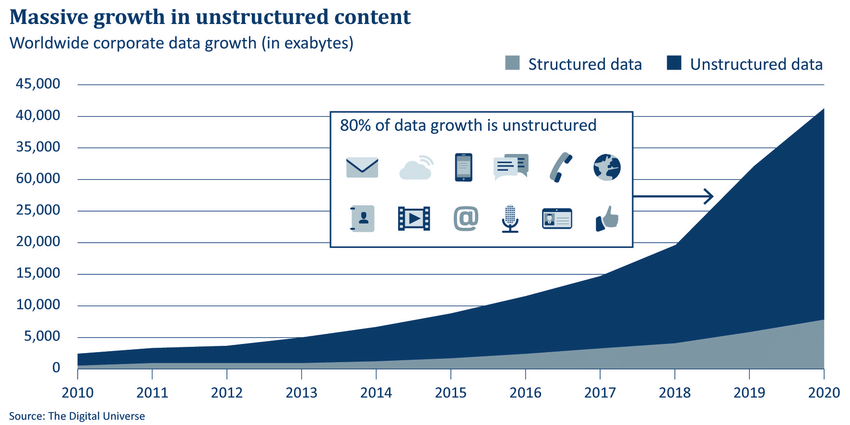
\includegraphics[width=0.85\textwidth]{figures/Growth-in-worldwide-stored-data.png}
\end{center}
\end{frame}

\begin{frame} %%%%%%%%%%%%%%%%%%%%%%%%%%%%%%
\frametitle{Outline}
\tableofcontents
\end{frame}

\section{XML --- The Extensible Markup Language}
%!TEX root = lec07_documents.tex

\begin{frame}{The Web As Of Not Too Long Ago}

HTML: HyperText Markup Language
\begin{itemize}[-,noitemsep,topsep=-5pt]
\item \alert{W3C Standard} implemented by most browsers
\item Still not fully supported across all platforms
\end{itemize}

\vskip1em

HTML enabled mass publishing of human-generated content (e.g., news, blogs, etc.) and server-generated content (by pulling data out of a relational database)
\begin{itemize}[-,topsep=-5pt]
\item PHP, JavaScript, ASP...
\end{itemize}

\vskip1em

HTML was designed to present content for  \textbf{human consumption}. That is, it specifies how to make content look nice on the browser, not what that content \textbf{means}.

\end{frame}

\lstset{
	style=markup,
    emph=[1]{%
        name,content
    },
    emphstyle=[1]{\color{sqlColor}}
}

\newsavebox\movieHMLexample
\begin{lrbox}{\movieHMLexample}
\begin{lstlisting}[style=markup]
<HTML>
 <head>
  <title>Movie List</title>
  <meta name="author" 
        content="John Smith">
 </head>
 <body>
  <h1> Movie List </h1>
  <p> <i> Ghostbusters </i> (1984)
     <br> <b> Ivan Reitman </b>
     <br> With Bill Murray, 
           Sigourney Weaver

  <p> <i> Groundhog Day </i> (1993)
     <br> <b> Harold Ramis </b>
     <br> With Bill Murray, 
           Andie MacDowell
 </body>
</HTML>
\end{lstlisting}
\end{lrbox}


\begin{frame}[fragile]{Markup Languages}

\vskip1em

\begin{columns}[onlytextwidth]
\begin{column}{0.55\textwidth}
Markup: annotations (tags) in a plain text document

\vskip1em
HTML's markup vocabulary is \textbf{fixed} and tags have \alert{pre-specified semantics}:
\begin{itemize}[-,noitemsep,topsep=-5pt]
\item \lstinline[style=markup]!<head>! tag is for metadata while the ``data'' goes into the \lstinline[style=markup]!<body>! tag.
\item HTML has tags for choosing fonts and colors, drawing tables, adding line breaks, paragraphs, hierarchical headers, etc.
\end{itemize}

\vskip1em
Tags need not be closed in HTML
\end{column}
\begin{column}{0.4\textwidth}
\begin{tikzpicture}
\node {\scalebox{0.85}{\usebox\movieHMLexample}};

\onslide<2-|handouts:1>{
  \node (markup) at (0,4) [color=blue] {markup};
  \node (c1) at (-1.75,3.5) [color=blue,circle] {};
  \node (c2) at (1,3) [color=blue,circle] {};
  \draw [blue,thick,->,>=stealth] (markup) -- (c1); \draw [blue,thick,->,>=stealth] (markup) -- (c2);
}
\onslide<3|handouts:1>{
  \node (content) at (1,1.5) [color=red] {content};
  \node (c3) at (-0.5,0.75) [color=blue,circle] {};
  \draw [red,thick,->,>=stealth] (content) -- (c3);
}
\end{tikzpicture}
\end{column}
\end{columns}

\end{frame}


\newsavebox\movieXMLexample
\begin{lrbox}{\movieXMLexample}
\begin{lstlisting}[style=markup]
<movies>
 <meta name="author" 
        content="John Smith"/>
 <movie>
  <title>Ghostbusters</title>
  <year>1984</year>
  <director>Ivan Reitman</director>
  <cast>
   <actor>Bill Murray</actor>
   <actor>Sigourney Weaver</actor>
  </cast>
 </movie>
 <movie>
  <title>Groundhog Day</title>
  <year>1993</year>
  <director>Harold Ramis</director>
  <cast>
     <actor>Bill Murray</actor>
     <actor>Andie MacDwowell</actor>
  </cast>
 </movie>
</movies>
\end{lstlisting}
\end{lrbox}

\begin{frame}[fragile]{The Extensible Markup Language}

\vskip2em
\begin{columns}[onlytextwidth]
\begin{column}{0.54\textwidth}
W3C~recommendation markup language that allows user-defined vocabulary.
\begin{itemize}[-,topsep=-5pt]
\item Programmers choose their own tags.
\item Applications can interpret the tags any way they want.
\end{itemize}

\vskip2em

XML tags must always be closed in the reverse order in which they are opened.
\begin{itemize}[-,topsep=-5pt]
\item Ensures the document can be parsed correctly.
\end{itemize}
\end{column}
\begin{column}{0.4\textwidth}
\scalebox{0.75}{\usebox\movieXMLexample}
\end{column}
\end{columns}
\end{frame}

\begin{frame}{XML vs HTML}

In summary:

\begin{itemize}[-]
\item Both are markup languages that apply to plain text documents
\item HTML has a finite and pre-defined set of tags; with XML, you can choose your own set of tags
\item HTML and XML documents can be represented as trees (through the Document Object Model)
\item Closing tags in HTML is optional; the browser makes educated guesses about the shape of the tree
\item Closing tags in XML is required; there is only one DOM tree that represents a well-formed XML document
\end{itemize}
\end{frame}


\begin{frame}{XML Standards}

XSL/XSLT: presentation and transformation
\begin{itemize}[-,topsep=-05pt,noitemsep]
\item ex: transforming XML into plain HTML content
\end{itemize}

RDF: resource description framework 
\begin{itemize}[-,topsep=-5pt,noitemsep]
\item used for describing meta-data about XML documents
\item foundation for the Semantic Web
\end{itemize}

Xpointer/Xlink: specifies links across documents and elements

DOM: Document Object Model for representing XML documents
\begin{itemize}[-,topsep=-5pt,noitemsep]
\item implementations in all popular languages
\end{itemize}


SAX: Simple API for XML parsing
\begin{itemize}[-,topsep=-5pt,noitemsep]
\item event-based framework
\item implementations in all popular languages
\end{itemize}
\end{frame}

\begin{frame}{What is XML good for?}

\begin{wrapfigure}[6]{r}{0.4\textwidth}
\vspace*{-3em}
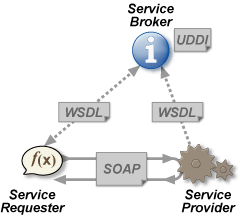
\includegraphics[width=0.4\textwidth]{figures/Webservices.png}
\end{wrapfigure}

\textbf{Web Services}\footnote{\url{https://en.wikipedia.org/wiki/Web_service}} are software systems designed to support interoperable machine-to-machine interaction over the Web (or some other network). 

With Service-Oriented Architectures, an entire application can be implemented by calling services that perform specific tasks.

XML is used to encode messages between the application (the requester) and the service provider. The application can choose among many providers offering the same service.

See CMPUT401!
\end{frame}


\begin{frame}{What is XML good for?}

\vskip1em

\begin{columns}[onlytextwidth]
\begin{column}{0.38\textwidth}
\textbf{Ajax}\footnotemark, short for asynchronous JavaScript and XML, is a set of web development techniques using many web technologies on the client side to create asynchronous web applications.

\vskip1em

See CMPUT404!
\end{column}
\begin{column}{0.6\textwidth}
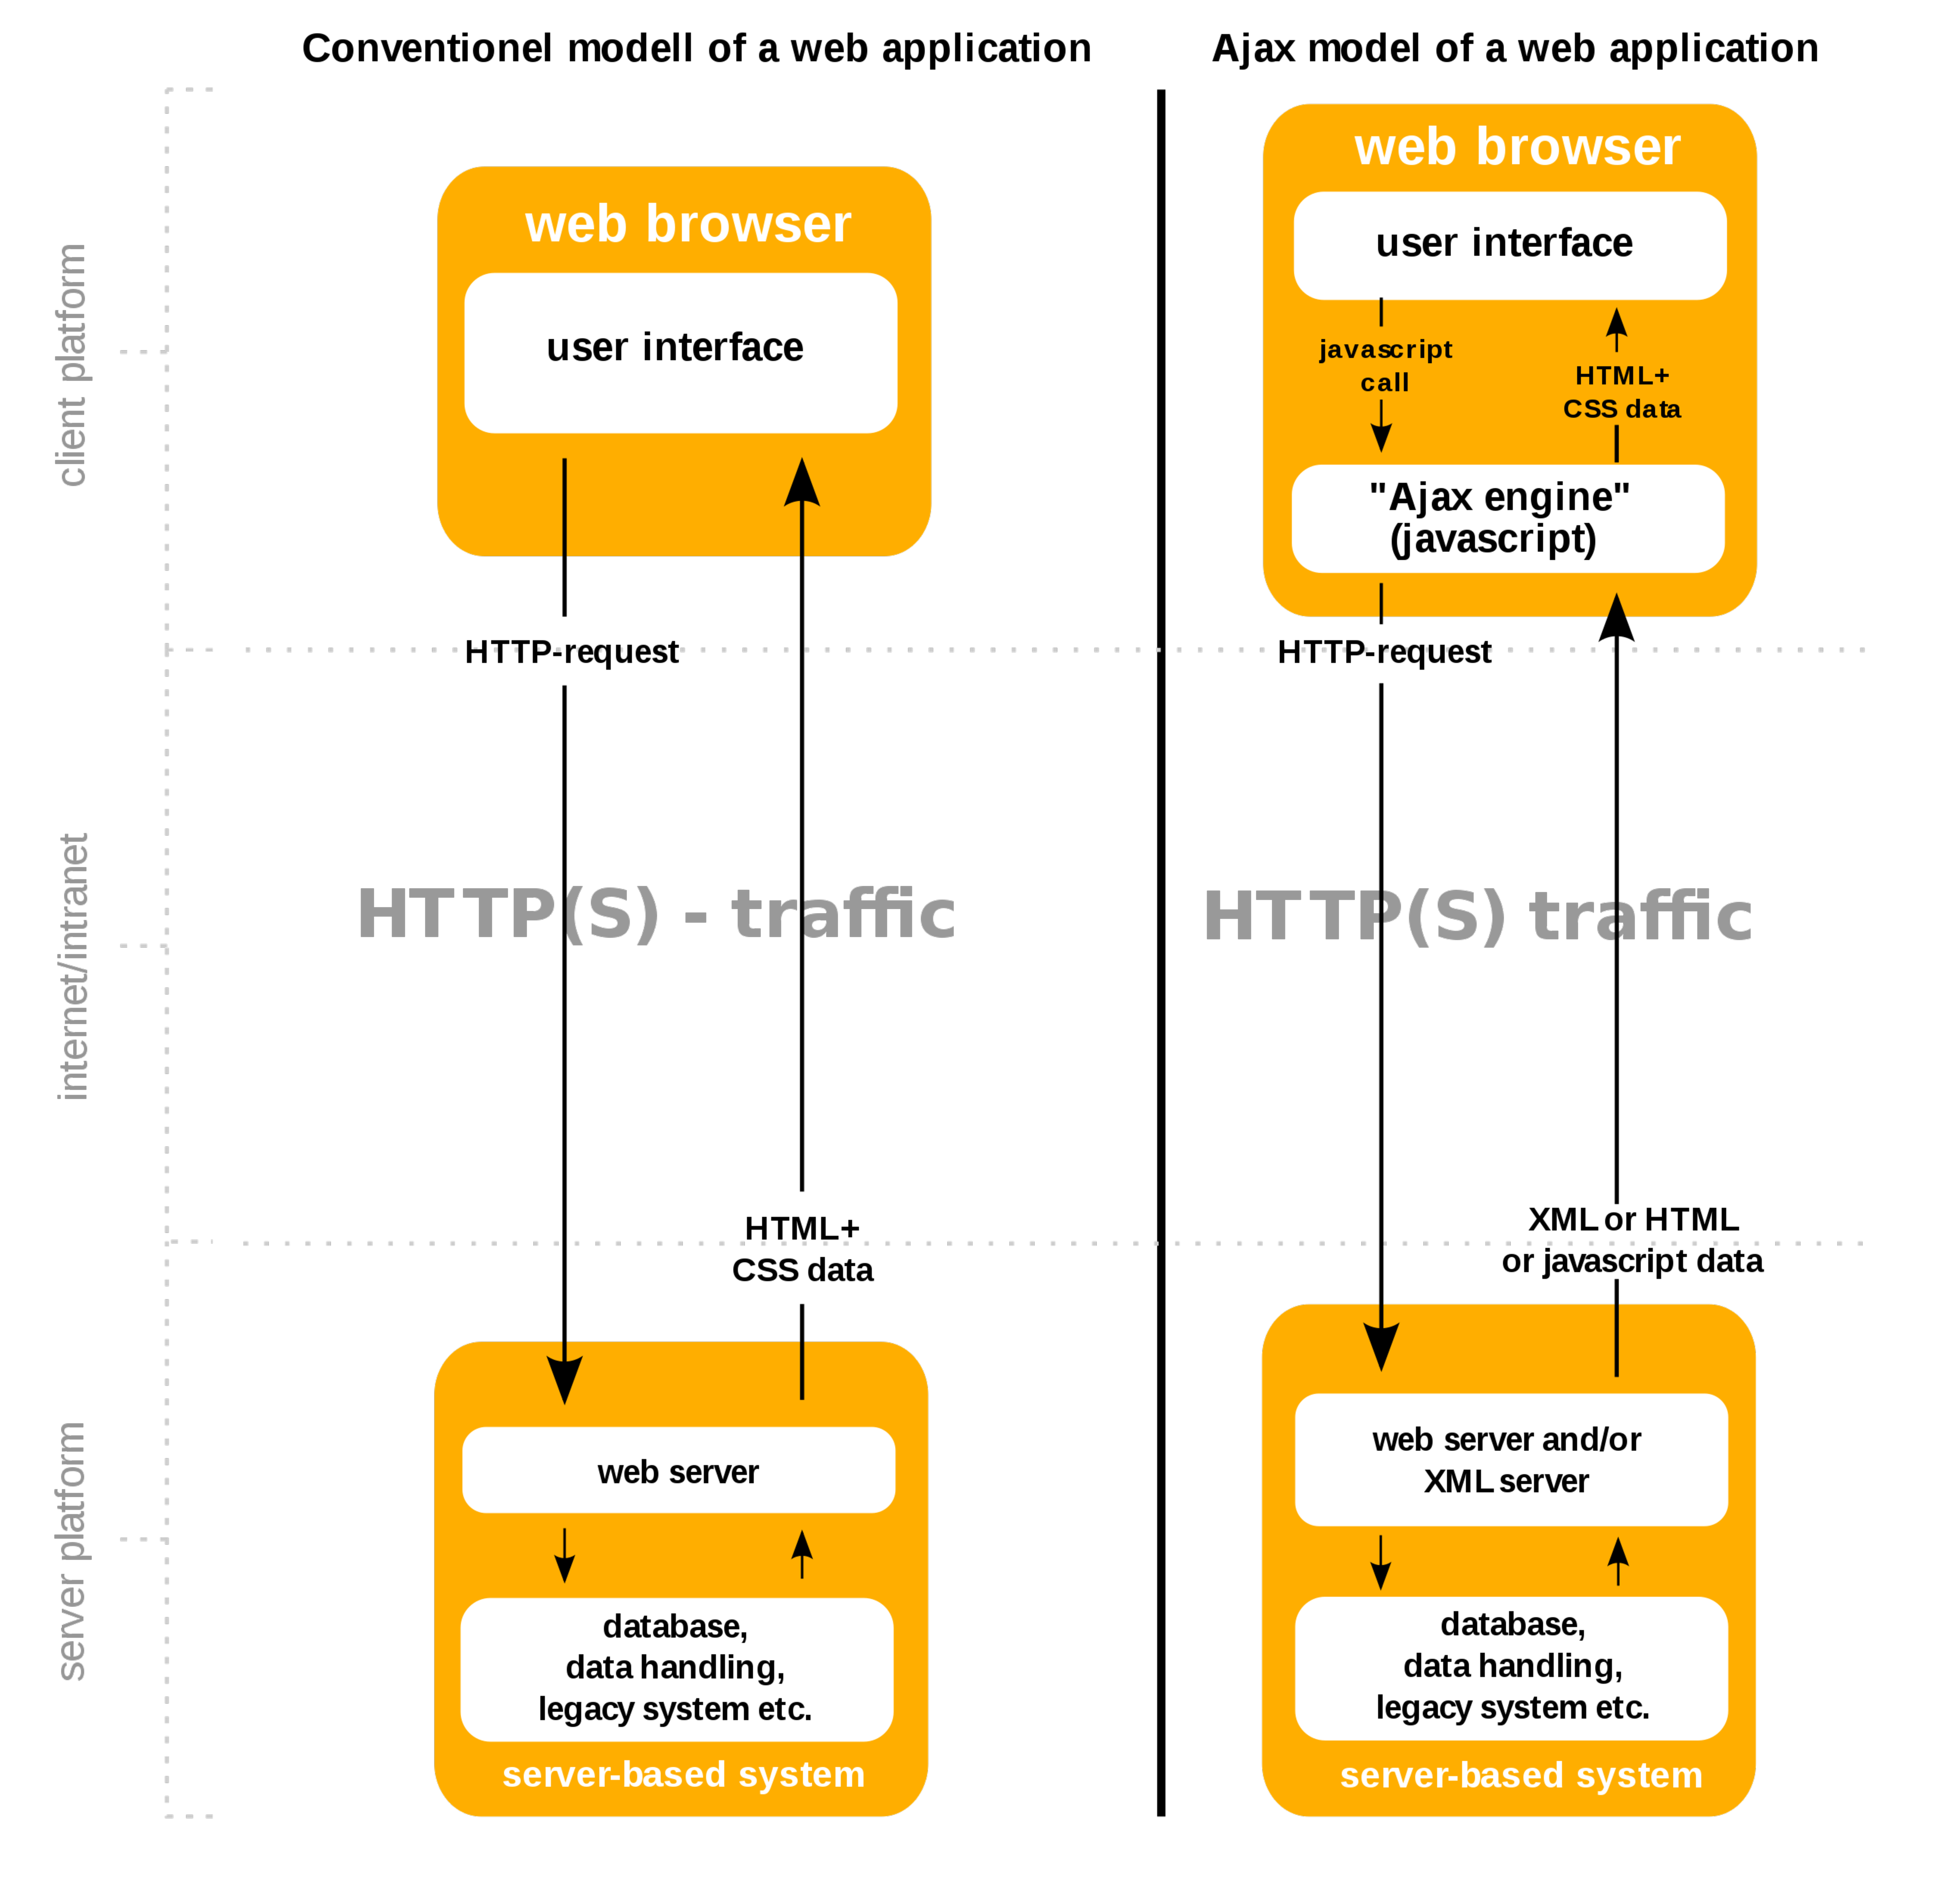
\includegraphics[width=1.2\textwidth]{figures/2560px-Ajax-vergleich-en.pdf}
\end{column}
\end{columns}

\footnotetext{\url{https://en.wikipedia.org/wiki/Ajax_(programming)}}
\end{frame}

\begin{frame}{What is XML good for?}

XML is great for \alert{encoding and exchanging data} \textbf{between} existing (database-backed) \textbf{systems}.

Why?
\begin{itemize}[-]
\item XML is \textbf{text-based}: it is a lot easier to read or write text files than binary files (e.g., the programmer can inspect the file while debugging).
\item It enables incremental data sharing formats; once two systems can talk, it is easy to extend the markup to support more systems.
\item XML is an open standard, supported by many tools (and developers).
\end{itemize}

\end{frame}

\newsavebox\exampleXMLDTD
\begin{lrbox}{\exampleXMLDTD}
\begin{lstlisting}[style=markup]
<?xml version="1.0" encoding="UTF-8"?>
<?xml-stylesheet type="text/css" href="movies.css"?>
<!DOCTYPE movies SYSTEM "http://movies.org/movies.dtd">
<movies>
 <movie> 
  <title>Ghostbusters</title> <year>1984</year>
  <director>Ivan Reitman</director>
  <cast>
    <actor>Bill Murray</actor>
<!-- this is a comment -->
    <actor>Sigourney Weaver</actor>
  </cast>
 </movie>
</movies>
\end{lstlisting}
\end{lrbox}


\begin{frame}[fragile]{What Does XML Look Like?}

\vspace*{-2em}
\begin{center}
\begin{tikzpicture}
\node (fig) at (0,0) [anchor=north west] {\scalebox{0.75}{\usebox\exampleXMLDTD}};
\node (c1) at (0.25,-0.25) [circle,blue] {};
\node (c2) at (0.25,-1) [circle,blue] {};
\node (c3) at (6,-0.6) [circle,blue] {};
\node (c4) at (0.25,-3.5) [circle,blue] {};
\node (enc) at (-2,0) [rectangle,draw,blue,align=center,text width=1.75cm] {\footnotesize encoding};
\draw[blue,thick,->,>=stealth] (enc) -- (c1);
\node (dtd) at (-2,-1) [rectangle,draw,blue,align=center,text width=1.75cm] {\footnotesize document\\[-0.75em] type};
\draw[blue,thick,->,>=stealth] (dtd) -- (c2);
\node (css) at (7,0.25) [rectangle,draw,blue,align=center,text width=1.75cm] {\footnotesize Stylesheet};
\draw[blue,thick,->,>=stealth] (css) -- (c3);
\node (com) at (-2,-3) [rectangle,draw,blue,align=center,text width=1.75cm] {\footnotesize comment};
\draw[blue,thick,->,>=stealth] (com) -- (c4);
\end{tikzpicture}
\end{center}

An XML element consists of an opening tag, the corresponding closing tag, and everything that goes in between them

The \alert{content of the element} is what goes between the tags\\
~$-$~~may consist of: text, other elements, or a mix of both

\end{frame}

\begin{frame}[fragile]{Representing relational data as XML}

XML is a quite popular format for exchanging relational data, because most applications use RDBMSs. In fact, there is even a standard called SQL/XML that helps with that. (More on this later).

\vskip1em

\begin{columns}[onlytextwidth]
\begin{column}{0.45\textwidth}
An obvious solution would be to map each row of each relation to an element:

\vskip1em

\scalebox{0.75}{\usebox\MovieTable}
\end{column}
\begin{column}{0.45\textwidth}
\begin{lstlisting}[style=markup,basicstyle=\ttfamily\scriptsize]
...
<Movie>
 <row> <title>Ghostbusters</title>
    <year>1984</year>
    <imdb>7.8</imdb>
    <director>Ivan Reitman</director>
 </row>
  <row> <title>Big</title>
  ... 
  </row>
 ...
</Movie>
...
\end{lstlisting}
\end{column}
\end{columns}
\end{frame}

\begin{frame}[fragile]
XML does not suffer from the 1NF limitation: elements can be multi-valued. Thus we can ``nest'' a table inside another (e.g., if there is a PK/FK relationship between them):

\begin{center}
\begin{lstlisting}[style=markup][basicstyle=\ttfamily\scriptsize]
...
<Movie>
 <row> <title>Ghostbusters</title>
    <year>1984</year>
    <imdb>7.8</imdb>
    <director>Ivan Reitman</director>
    <cast>
      <actor>Bill Murray</actor> <role>Dr. Venkman</role>
      <actor>Sigourney Weaver</actor> <role>Dana Barret</role>
    </cast>
 </row>
 ...
</Movie>
...
\end{lstlisting}
\end{center}

\end{frame}

\begin{frame}[fragile]{Attributes, data and meta-data}

\begin{center}
\footnotesize
\begin{lstlisting}[style=markup]
<bibliography> 
   <book -|isbn|-="046509760X">
        <title>The Book of Why</title>
        <author>Pearl</author>
        <author>Mackenzie</author>
        <publisher>Basic Books</publisher>
        <price -|currency|-="CDN">45.00</price>
   </book>
</bibliography>
\end{lstlisting}
\end{center}

Attributes may be added to describe, identify or \alert{link} elements
\begin{itemize}[-,noitemsep]
\item \lstinline{-|isbn|-} identifies the book
\item \lstinline{-|currency|-} explains that the price is in Canadian dollars
\end{itemize}

In principle, attributes should be \emph{metadata}; but it is hard to distinguish data from metadata sometimes.
\end{frame}



\newsavebox\PandPXML
\begin{lrbox}{\PandPXML}
\begin{lstlisting}[style=markup][linewidth=0.7\textwidth,breaklines=true]
<book>
 <title>Pride And Prejudice</title>
 <chapter>
  <title>Chapter 1</title>
  <p>It is a truth universally acknowledged, 
  that a single man in possession of a good 
  fortune must be in want of a wife. </p>
  <p>...</p>
  ...
 </chapter>
 <chapter>
  <title>Chapter 2</title>
  <p>Mr. Bennet was among the earliest of 
  those who waited on Mr. Bingley...</p>
  <p>...</p>
  ...
 </chapter>
 ...
</book>
\end{lstlisting}
\end{lrbox}

\begin{frame}[fragile]{Document Order}

\vskip2em

\begin{columns}[onlytextwidth]
\begin{column}{0.5\textwidth}
XML is meant to encode \alert{documents}, thus, unlike with tuples in a table, the ordering of the elements in a document is important.
\begin{itemize}[-,topsep=-0.5pt,noitemsep]
\item Think about reading your favorite book in a random order of chapters!
\item XML Storage systems must preserve element ordering.
\end{itemize}

\vskip1em

As we will see later, we can ask queries involving element order.

\end{column}
\begin{column}{0.45\textwidth}
\scalebox{0.75}{\usebox\PandPXML}
\end{column}
\end{columns}
\end{frame}

\begin{frame}[fragile]{XML Elements are Trees}

The nesting of elements naturally induce a tree, often called the Document Object Model (DOM) tree:

\begin{lstlisting}[style=markup][basicstyle=\ttfamily\scriptsize]
   <book>
        <title>The Book of Why</title>
        <author>Pearl</author>
        <author>Mackenzie</author>
        <publisher>Basic Books</publisher>
   </book>
\end{lstlisting}

\small
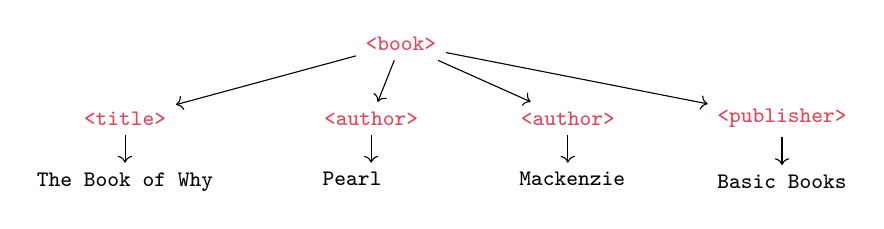
\begin{tikzpicture}[every node/.style={font=\footnotesize\ttfamily}]
\node (book) at (0,0) {\textcolor{accent}{<book>}};
\node (title) [below left=15pt and 65pt of book] {\textcolor{accent}{<title>}};
\node (a1) [right= 50pt of title] {\textcolor{accent}{<author>}};
\node (a2) [right= 30pt of a1] {\textcolor{accent}{<author>}};
\node (publisher) [right= 30pt of a2] {\textcolor{accent}{<publisher>}};
\node (t) [below= 10pt of title] {The Book of Why};
\node (at1) [below= 10pt of a1,text width=35pt] {Pearl};
\node (at2) [below= 10pt of a2,text width=35pt] {Mackenzie};
\node (p) [below= 10pt of publisher] {Basic Books};
\draw[->] (book) -- (title); \draw[->] (book) -- (a1); \draw[->] (book) -- (a2); \draw[->] (book) -- (publisher);
\draw[->] (title) -- (t);
\draw[->] (a1) -- (at1); \draw[->] (a2) -- (at2); \draw[->] (publisher) -- (p);
\end{tikzpicture}

Edges in the tree represent the \textbf{parent-child} relationship, from which we can derive other relationships: ancestor, descendant and sibling.

\end{frame}



\begin{frame}[fragile]{Constraints? Schemas?}

\begin{BOX}{Document Type Definitions (DTDs)}
Originated from SGML\footnotemark; uses \alert{regular expressions} to specify which elements can be nested within others and simple rules to specify attributes.
\end{BOX}

\footnotetext{Standard Generalized Markup Language--\url{https://en.wikipedia.org/wiki/Standard_Generalized_Markup_Language}}


\begin{BOX}{XML Schema}
Borrow best practices from databases and programming languages; adds support for specifying data types for the various elements.

\vskip0.5em

Strictly more powerful than DTDS: you can always rewrite a DTD as a schema, but not the other way around.
\end{BOX}
\end{frame}


\lstset{language=DTD}

\newsavebox\DTDexample
\begin{lrbox}{\DTDexample}
\begin{lstlisting}
<!DOCTYPE bibliography [
 <!ELEMENT bibliography (book-|*|-)>
 <!ELEMENT book (title, author-|+|-, publisher, price-|?|-)>
 <!ATTLIST book isbn -:ID #REQUIRED:->
 <!ELEMENT title (-:#PCDATA:-)>
 <!ELEMENT author (-:#PCDATA:-)>
 <!ELEMENT publisher (-:#PCDATA:-)>
 <!ELEMENT price (-:#PCDATA:-)
 <!ATTLIST price currency -:CDATA #IMPLIED:-> 
]>
\end{lstlisting}
\end{lrbox}


\begin{frame}[fragile]{DTDs}

\vskip1em

\begin{columns}[onlytextwidth]
\begin{column}{0.35\textwidth}
\lstinline{ELEMENT} rules specify what can go in an element via \alert{regular expressions}.

\vspace*{2em}
\end{column}
\begin{column}{0.6\textwidth}
\scalebox{0.8}{\usebox\DTDexample}
\end{column}
\end{columns}


Each \lstinline{bibliography} element can contain zero or more \lstinline{book} elements and nothing else.

A \lstinline{book} element \textbf{must} have a \lstinline{title}, at least one \lstinline{author}, and a \lstinline{publisher}; it may also have a \lstinline{price} element.

Elements \lstinline{title}, \lstinline{author}, \lstinline{publisher}, and \lstinline{price} can contain only ``parsed character data'' (\lstinline[language=DTD]!-:#PCDATA:-!), which is XML for ``text''.

\end{frame}

\begin{frame}[fragile]{Validation of \lstinline{ELEMENT} Rules}

\textbf{Defn}: an element is valid if its \emph{content} matches the regular expression associated with its name in the DTD.

\textbf{Defn}: a document is valid if all of its elements are valid.


For validation purposes, the \emph{content} of element $x$ is one of\footnote{XML allows elements to have \emph{mixed} content as well: that is, elements interspersed with text. We will ignore such content in CMPUT391 for simplicity.}:\\
 - a string formed by the labels of the children of $x$\\
 - \lstinline[language=DTD]{-:#PCDATA:-} if the element contains only text

\begin{block}{Example: \lstinline[style=markup]{<cast><actor>Bill Murray</actor></cast>}}
The content of the \lstinline[style=markup]{<cast>} element is \lstinline[style=markup]{actor}, and the content of \lstinline[style=markup]{<actor>} is \lstinline[language=DTD]{-:#PCDATA:-}.
\end{block}
\end{frame}

\begin{frame}[fragile]

\vskip2em

\begin{lstlisting}[style=markup][basicstyle=\ttfamily\scriptsize]
<bibliography>
    <book>
        <title>The Book of Why</title>
        <author>Pearl</author>
        <author>Mackenzie</author>
        <publisher>Basic Books</publisher>
    </book>
</bibliography>
\end{lstlisting}

% \small
% \begin{tikzpicture}[every node/.style={font=\footnotesize\ttfamily}]
% \node (book) at (0,0) {\textcolor{accent}{<book>}};
% \node (title) [below left=15pt and 65pt of book] {\textcolor{accent}{<title>}};
% \node (a1) [right= 50pt of title] {\textcolor{accent}{<author>}};
% \node (a2) [right= 30pt of a1] {\textcolor{accent}{<author>}};
% \node (publisher) [right= 30pt of a2] {\textcolor{accent}{<publisher>}};
% \node (t) [below= 10pt of title] {The Book of Why};
% \node (at1) [below= 10pt of a1,text width=35pt] {Pearl};
% \node (at2) [below= 10pt of a2,text width=35pt] {Mackenzie};
% \node (p) [below= 10pt of publisher] {Basic Books};
% \draw[->] (book) -- (title); \draw[->] (book) -- (a1); \draw[->] (book) -- (a2); \draw[->] (book) -- (publisher);
% \draw[->] (title) -- (t);
% \draw[->] (a1) -- (at1); \draw[->] (a2) -- (at2); \draw[->] (publisher) -- (p);
% \end{tikzpicture}

\vskip2em

Is the element above valid?

\begin{lstlisting}[basicstyle=\ttfamily\scriptsize]
 <!ELEMENT bibliography (book-|*|-)>
 <!ELEMENT book (title, author-|+|-, publisher, price-|?|-)>
 <!ELEMENT title (-:#PCDATA:-)>
 <!ELEMENT author (-:#PCDATA:-)>
 <!ELEMENT publisher (-:#PCDATA:-)>
 <!ELEMENT price (-:#PCDATA:-)
\end{lstlisting}

\end{frame}

\begin{frame}[fragile]

\vskip1em

\begin{columns}[onlytextwidth]
\begin{column}{0.35\textwidth}
\lstinline{ATTLIST} rules specify whether attributes are required, and whether they can be used as identifiers.

\vspace*{2em}
\end{column}
\begin{column}{0.6\textwidth}
\scalebox{0.8}{\usebox\DTDexample}
\end{column}
\end{columns}


\lstinline[language=DTD]!-:CDATA:-! means ``character data''. Attributes cannot have elements or other attributes as their value.

\lstinline[language=DTD]!-:#REQUIRED:-! indicates the attribute must be present; while \lstinline[language=DTD]!-:#IMPLIED:-! means the attribute is optional.

Finally, \lstinline[language=DTD]!-:#ID:-! indicates that the value of the attribute must be unique \textbf{within the document}.

\end{frame}


\newsavebox\bibliographyDTD
\begin{lrbox}{\bibliographyDTD}
\begin{lstlisting}[language=DTD,basicstyle=\ttfamily\scriptsize]
<!DOCTYPE bibliography [
 <!ELEMENT bibliography (book-|*|-)>
 <!ELEMENT book (title, author-|+|-, publisher, price-|?|-)>
 <!ATTLIST book isbn ID #REQUIRED
                -|sequel IDREF|- #IMPLIED>
 <!ELEMENT title (#PCDATA)>
 <!ELEMENT author (#PCDATA)>
 <!ELEMENT publisher (#PCDATA)>
 <!ATTLIST -|publisher website|- ID #IMPLIED>
 <!ELEMENT price (#PCDATA)
 <!ATTLIST price currency CDATA #IMPLIED> 
]>
\end{lstlisting}
\end{lrbox}

\begin{frame}[fragile]{\lstinline[language=DTD]!-:ID:-! and \lstinline[language=DTD]!-:IDREF:-! attributes}

\lstinline[language=DTD]!-:#ID:-! and \lstinline[language=DTD]!-:#IDREF:-! attributes are ``like'' keys and foreign keys, but not quite, because their scope is the entire document (instead of individual tables).

\vskip1em

\usebox\bibliographyDTD

% \lstset{language=DTD}

The (optional) \lstinline[language=DTD]!-|sequel|-! must match the value of some \lstinline[language=DTD]!-:#ID:-! attribute.
\end{frame}


\newsavebox\validATTexample
\begin{lrbox}{\validATTexample}
\begin{lstlisting}[style=markup]
<bibliography>
 <book isbn="1234"> 
  ...
  <publisher website="abc.ca">
   ...
  </publisher>
 </book>
 <book isbn="5678" sequel="1234">
  ...
  <publisher>...</publisher>
 </book>
 <book isbn="xyz" sequel="abc.ca">
  ...
 </book>
<bibliogaphy>
\end{lstlisting}
\end{lrbox}

\newsavebox\dtdATTexample
\begin{lrbox}{\dtdATTexample}
\begin{lstlisting}[language=DTD]
<!DOCTYPE bibliography [
 ...
 <!ATTLIST book isbn -:ID #REQUIRED:-
                -|sequel IDREF #IMPLIED|->
 <!ATTLIST -|publisher website ID #IMPLIED|->
 <!ATTLIST price currency -:CDATA #IMPLIED:-> 
]>
\end{lstlisting}
\end{lrbox}


\begin{frame}[fragile]{Validation of \lstinline[language=DTD]!ATTLIST! Rules}

A \lstinline[language=DTD]!-:#REQUIRED:-! attribute must be present, otherwise the element (and the document) is invalid. An \lstinline[language=DTD]!-:#IMPLIED:-! attribute is optional.

The value of an \lstinline[language=DTD]!-:#ID:-! attribute be unique within the document, while the value of an \lstinline[language=DTD]!-:#IDREF:-! attribute must match some \lstinline[language=DTD]!-:#ID:-! attribute.

\vskip1em

\begin{columns}[onlytextwidth]
\begin{column}{0.5\textwidth}
\scalebox{0.75}{\usebox\dtdATTexample}

\vskip1em

Note that, counter to what you would expect, we cannot specify that \lstinline!-|sequel|-! must match the \lstinline!-|isbn|-! of another book!
\end{column}
\begin{column}{0.4\textwidth}
\scalebox{0.75}{\usebox\validATTexample}
\end{column}
\end{columns}

\end{frame}


\begin{frame}{DTDs}

DTDs are enough for describing documents, but have many shortcomings if used to describe relational data.

\begin{itemize}[-]
\item Can ``simulate'' unary keys (ID attributes), but there is no support for n-ary keys.

\item No support for inclusion dependencies; IDREF attributes are not restricted to specific ID attributes.

\item Only data type is ``text''.

\item Element name and ``type'' (regular expression on child labels) are associated globally (i.e., independently of context).

\end{itemize}
\end{frame}

\begin{frame}[fragile]{XML Schema}
\begin{itemize}[-]
\item In XML format.
\item Element types are contextualized.\\
 - Ex: different book elements may have different types depending on the label of their parent.
\item Defines several primitive data types (integers, strings, dates, etc.) and allows user-defined data types.
\item Supports all common data types and the specification of domains (like SQL CHECK constraints)
\item Supports proper keys (including n-ary) and foreign keys.
\item Inheritance (extension or restriction).
\item Element-type reference constraints.
\end{itemize}
\end{frame}

\begin{frame}[fragile]{(Simplified) Example XML Schema}

\begin{lstlisting}[style=markup,basicstyle=\ttfamily\scriptsize]
<schema version="1.0" xmlns="http://www.w3.org/1999/XMLSchema">
 <element name="book">
   <complexType>
     <attribute name="isbn" type="string" use="required"/>
     <element name="title" type="string"/>
 
     <element name="author" minOccurs="1" maxOccurs="7" type="author_type"/>

      <element name="publisher" type="string" />

      <element ref="price" minOccurs="0" maxOccurs="1">
       <complexType>
          <simpleContent>
            <extension base="float"/>
            <attribute name="currency" type="string" use="optional"/>
          </simpleContent>
       </complexType>
      </element>
     </complexType>
 </element>
</schema>
\end{lstlisting}

\end{frame}

\section{XML Query Languages}
%!TEX root = lec07_documents.tex

\newsavebox\bibliographyOne
\begin{lrbox}{\bibliographyOne}
\begin{lstlisting}[style=markup]
<bibliography>
  <book>
    <title>The Book of Why</title>
    <author>Perl</author>
    <author>Mackenzie</author>
    <publisher>Basic Books</publisher>
    <year>2018</year>
  </book>
  <book>
    <title>The Art of Computer Programming</title>
    <author>
      <first>Donald</first>
      <last>Knuth</last>
    </author>
    <published>Addison-Wesley, 1969</published>
  </book>
</bibliography>
\end{lstlisting}
\end{lrbox}

\begin{frame}
Example XML document for the next few slides:

\begin{center}
\begin{tikzpicture}[every node/.style={inner sep=0,outer sep=0}]
\node<+-> at (0,0) [anchor=south west] {\scalebox{0.75}{\usebox{\bibliographyOne}}};

\begin{scope}[on background layer]
\onslide<2|handouts:1>{
  \fill [orange!10] (0.35,1) rectangle (3.5,2.35);
  \draw [->,red,thick] plot [smooth] coordinates {(0.35, 1.8) (-0.5,2.2) (-0.5, 4) (0.35, 4.4)};
  \node [red, anchor=east] at (-0.65,2.75) {($\dagger$)};
}
\onslide<3|handouts:1>{
  \fill [blue!10] (0.35,0.65) rectangle (6,0.975);
  \draw [->,blue,thick] plot [smooth] coordinates {(6, 0.8) (6.5,1.2) (6.5, 3) (5, 3.4)};
  \node [blue, anchor=west] at (6.75,2) {($\ddagger$)};
}
\end{scope}
\end{tikzpicture}
\end{center}

\uncover<+->{
\begin{itemize}[noitemsep]
\onslide<2-3|handouts:1>{\item[\textcolor{red}{($\dagger$)}] Elements need not have the same kind of content!}
\onslide<3|handouts:1>{\item[\textcolor{blue}{($\ddagger$)}] Missing or new elements are also possible.}
\end{itemize}}

\end{frame}

\begin{frame}{Data Model}

XML elements (including the entire document) are modeled as \textbf{ordered labeled trees}.

\begin{center}
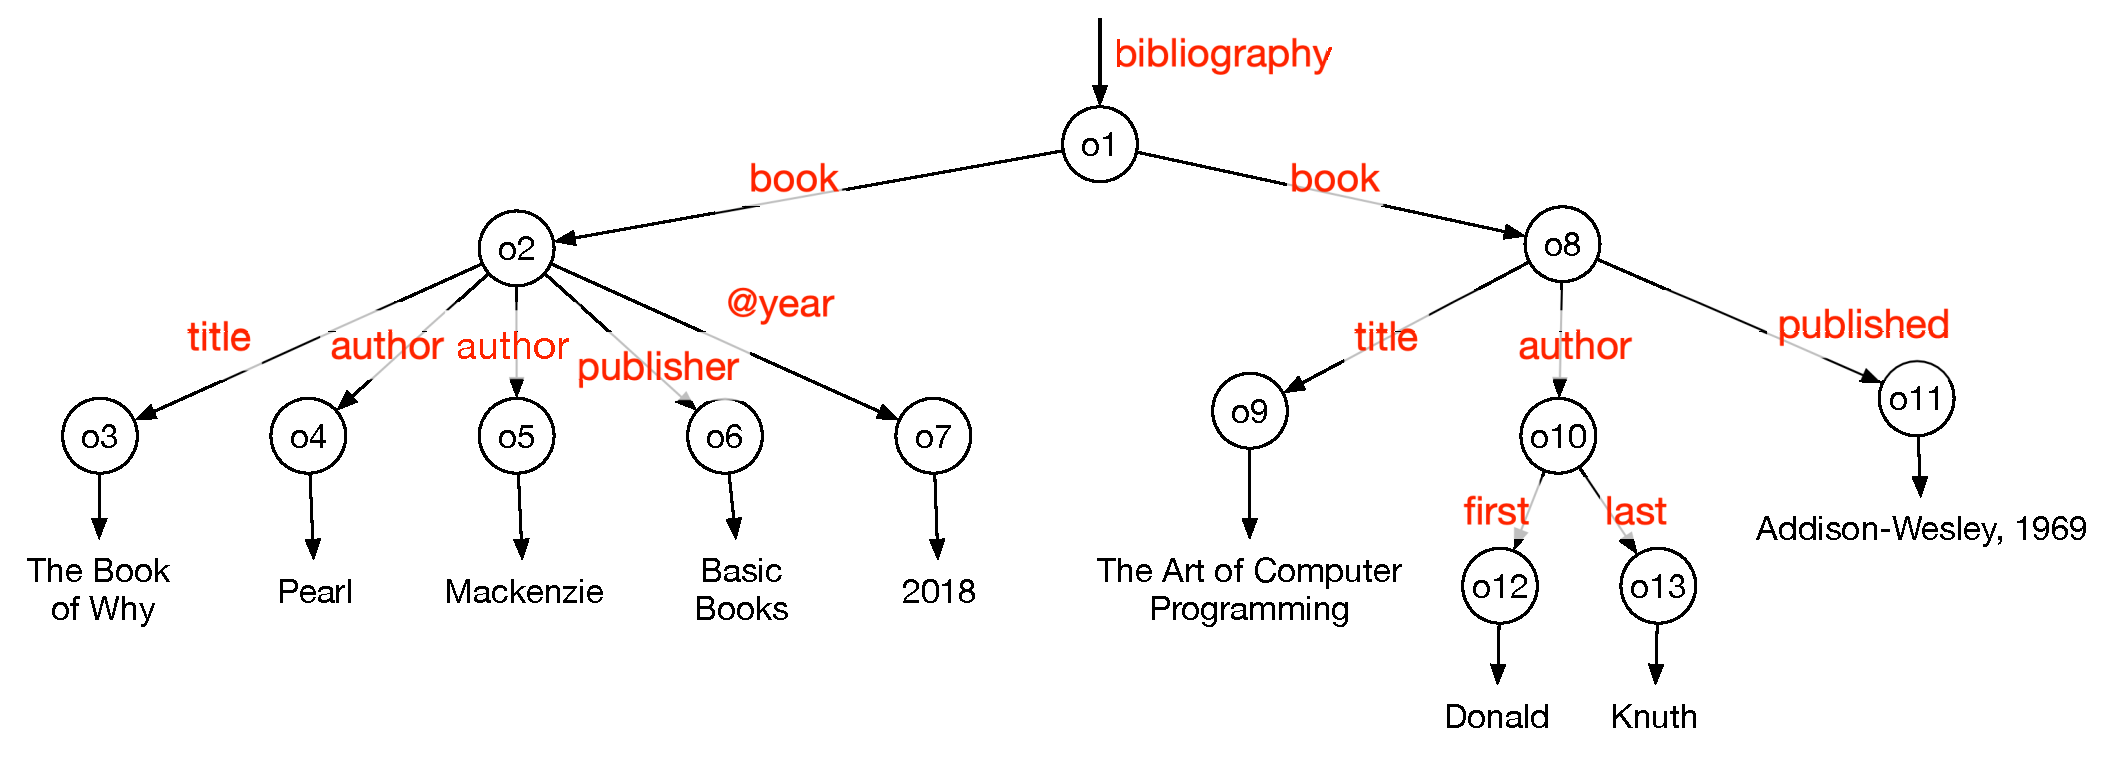
\includegraphics[width=\textwidth]{figures/XML_data_model.eps}
\end{center}

\vskip1em

XML is a \textbf{semi-structured} data format: different elements with the same label can have different types or different kinds of content.

\end{frame}

\begin{frame}{XML Query Languages}

The W3C defines (at least) two query languages for XML, which are used \textbf{together}. 

\begin{BOX}{XPath}
\begin{itemize}[-,noitemsep]
\item like regular expressions, but on paths over XML trees
\item specifies and ``returns'' nodes in the tree
\end{itemize}
\end{BOX}

\begin{BOX}{XQuery}
\begin{itemize}[-,noitemsep]
\item functional query language that computes an answer from input XML documents
\item uses XPath to locate nodes in the input (like the \lstinline{WHERE} clause in SQL) that are used to compute the answer
\end{itemize}
\end{BOX}

\end{frame}

\begin{frame}[fragile]{XPath}

XPath is a language for \textbf{addressing} parts of an XML document, designed to be used by both XSLT and XPointer. (\url{https://www.w3.org/TR/1999/REC-xpath-19991116/})

\begin{itemize}[-,topsep=-5pt,noitemsep]
\item Contains approximately 200 built-in functions.
\item A major element in the XML ecosystem, including XSLT, XLink, and XQuery.
\end{itemize}

\vskip1em

\lstset{language=XPath}

Every XPath expression returns \textbf{\alert{an ordered sequence}} of nodes in the XML tree. 

Unless otherwise specified, the ordering of the nodes is the \emph{document ordering}.

\end{frame}


\begin{frame}{XPath}

An XPath expression is a called a \alert{location \textbf{path}}:

\begin{block}{\alert{Location Path}}
A location path is a \textbf{sequence} of \blue{location \textbf{steps}}, separated by \alert{/}, that identifies one or more nodes in a \textbf{document}.
\end{block}

\vskip1em

\textbf{Example:} \fbox{\lstinline[style=XQuery]!doc("books.xml")/child::bibliography/child::book!}

\vskip1em

Each \textbf{Location \blue{Step}}:
\begin{itemize}[-,noitemsep,nolistsep,topsep=-0.5em]
\item Specifies a single navigational step in a path;
\item Is evaluated against a single \alert{context node}, and returns a \alert{\textbf{sequence} of nodes};
\item Almost always consists of a \alert{navigational axis} and a \alert{node test}.
\end{itemize}


\end{frame}

\begin{frame}[fragile]{Location Steps}

\textbf{Formally}: \fbox{\lstinline[style=XQuery]{axis::node test-:[:-predicate-:]:-}}
\begin{itemize}[-,noitemsep,topsep=-0.5em]
\item \textbf{Node tests} are optional. Often they are \alert{name tests} (i.e., an element or attribute name).

\item \textbf{Predicates} are also optional, and are used to filter nodes reachable using the axis and satisfying the name test.

\end{itemize}

\vskip1em

Most \textbf{common axes} and their \textbf{abbreviated forms}:
\begin{center}
\begin{tabular}{c|c|l}
axis & abbreviation & example\\
\hline
child & \lstinline[style=XQuery]!-:/:-! & \lstinline[style=XQuery]!doc("books.xml")-:/:-bibliography! \\
descendant-or-self & \lstinline[style=XQuery]!-://:-! & \lstinline[style=XQuery]!doc("books.xml")-://:-book! \\
attribute & \lstinline[style=XQuery]!-:@:-! & \lstinline[style=XQuery]!//book/-:@:-year! \\
self & \lstinline[style=XQuery]!-:.:-! & \lstinline[style=XQuery]!//author[-:.:-/last = 'Knuth']! \\
ancestor & \lstinline[style=XQuery]!-:..:-! & \lstinline[style=XQuery]!//first[-:..:-/last = 'Knuth']!
\end{tabular}
\end{center}


\end{frame}

\begin{frame}[fragile]

\lstset{language=XPath}

\hspace*{-2em}
\begin{tikzpicture}
\node at (0,0) [anchor=south west] {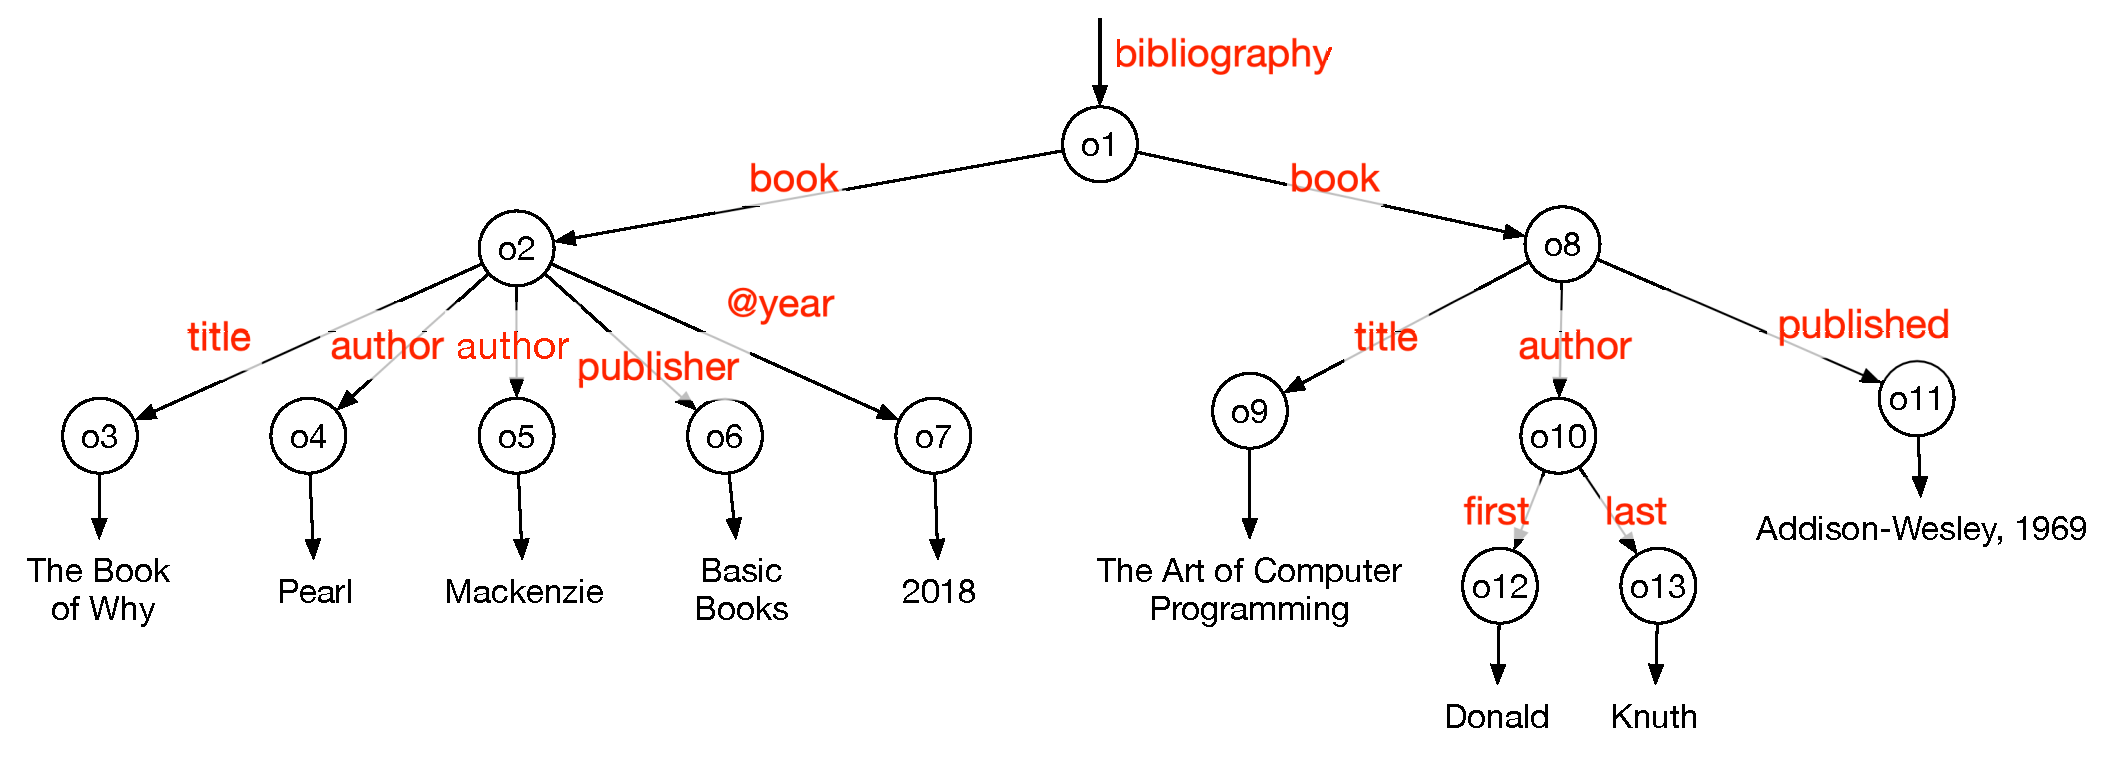
\includegraphics[width=1.1\textwidth]{figures/XML_data_model.eps}};

\node (p1) at (0,-1) [anchor=west] {\lstinline[style=Xquery]{/bibliography/book/@year}  = };
\node (p2) at (0,-2) [anchor=west] {\lstinline[style=Xquery]{/bibliography//author}  =  };
\node (p3) at (0,-3) [anchor=west] {\lstinline[style=Xquery]{//first/../author}  = };
\onslide<2-| handout:1>{\node [blue,yshift=2pt,right= 0.25cm of p1] {( o7 )};}
\onslide<3-| handout:1>{\node [blue,yshift=2pt,right= 0.25cm of p2] {( o4, o5, o10 )};}
\onslide<4-| handout:1>{\node [blue,yshift=2pt,right= 0.25cm of p3] {( o10 )};}
\end{tikzpicture}
\end{frame}


\newsavebox\personXML
\begin{lrbox}{\personXML}
\begin{lstlisting}[style=markup]
<?xml version="1.0"?>
<people>
  <person born="1912" died="1954">
    <name>
      <first>Alan</first>
      <last>Turing</last>
    </name>
    <profession>computer scientist</profession>
    <profession>mathematician</profession>
    <profession>cryptographer</profession>
  </person>
  <person born="1918" died="1988">
    <name>
      <first>Richard</first>
      <middle_initial>P</middle_initial>
      <last>Feynman</last>
    </name>
    <profession>physicist</profession>
    <hobby>Playing the bongoes</hobby>
  </person>
</people>
\end{lstlisting}
\end{lrbox}


\begin{frame}{Comparison Expressions}

XPath and XQuery model XML have multiple comparators.

\begin{center}
\begin{tabular}{c|c|c}
\blue{General} & \alert{Value} & \\
\blue{Comparator} & \alert{Comparator} & \raisebox{0.5em}{Description} \\
\hline
\lstinline[style=XQuery]{-:=:-} & \lstinline[style=XQuery]{eq} & Equals\\
\lstinline[style=XQuery]{-:!=:-} & \lstinline[style=XQuery]{ne} & Not equals\\
\lstinline[style=XQuery]{-:>:-} & \lstinline[style=XQuery]{gt} & Greater than \\
\lstinline[style=XQuery]{-:>=:-} & \lstinline[style=XQuery]{ge} & Greater than or equals to\\
\lstinline[style=XQuery]{-:<:-} & \lstinline[style=XQuery]{lt} & Less than\\
\lstinline[style=XQuery]{-:<=:-} & \lstinline[style=XQuery]{le} & Less than or equals to
\end{tabular}
\end{center}

\vskip1em

\blue{General} comparators can be used to compare \blue{values and sequences}, while \alert{value} comparators can \alert{only} be used to compare two \alert{values}.

\end{frame}


\begin{frame}[fragile]

\hspace*{-2em}
\begin{tikzpicture}
\node at (0,0) [anchor=south west] {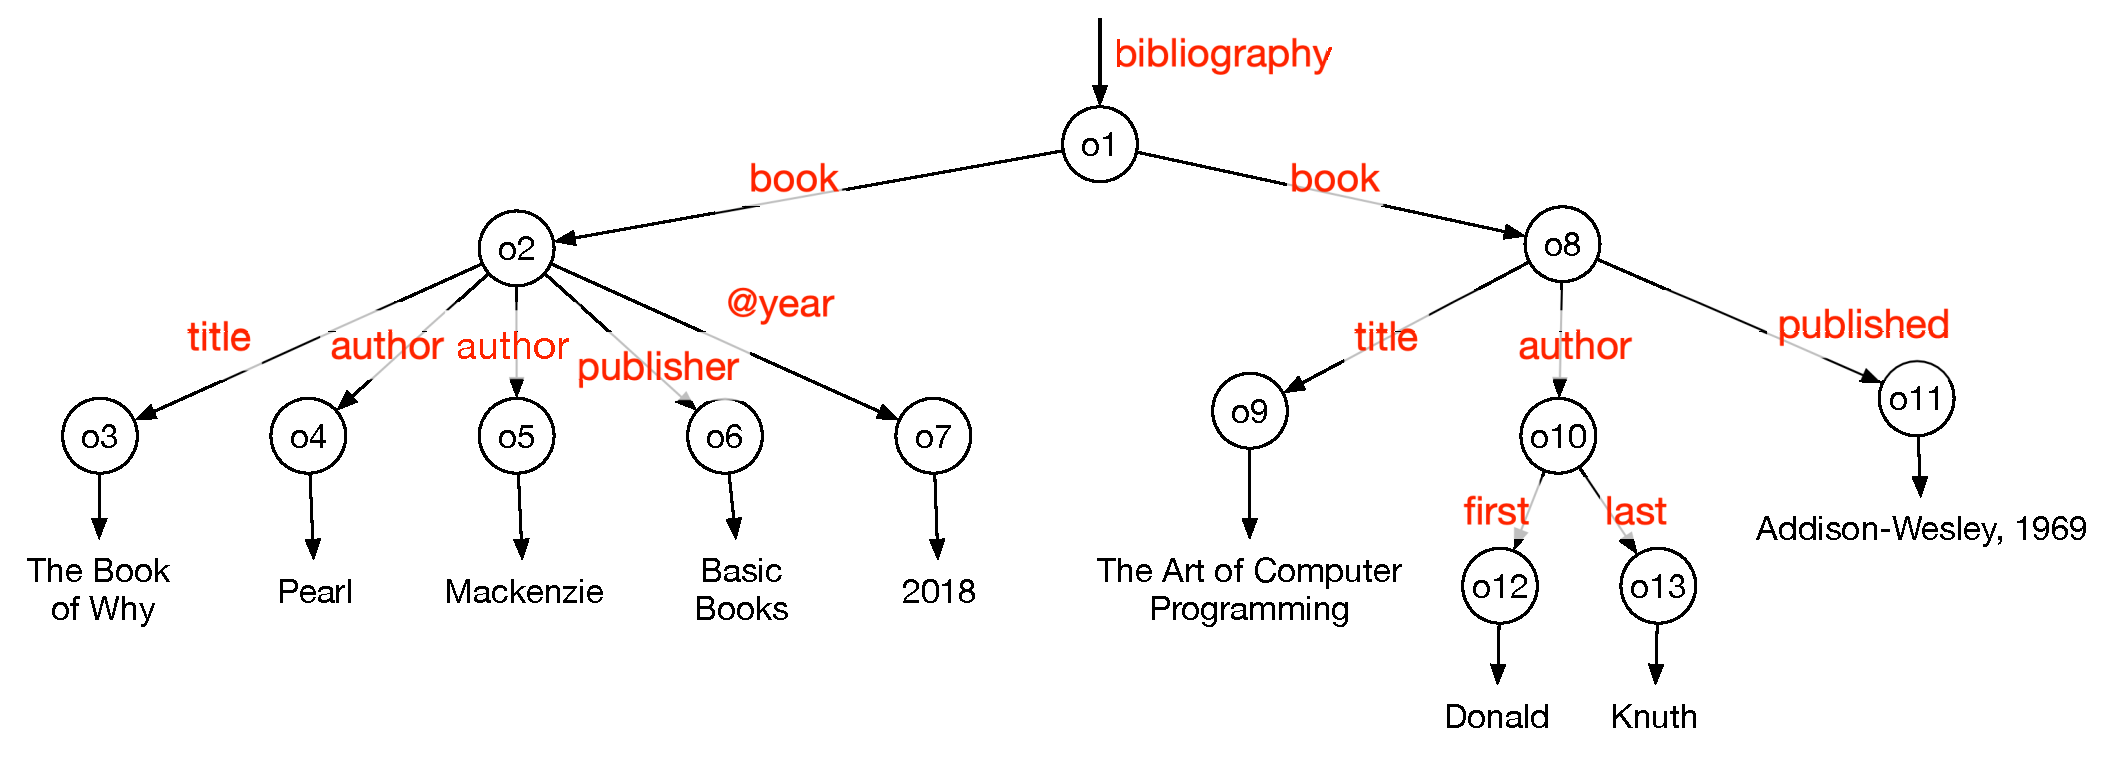
\includegraphics[width=1.1\textwidth]{figures/XML_data_model.eps}};
\end{tikzpicture}

\textbf{Example}: selecting books  written by \lstinline[style=XQuery]{Pearl}... because there can be many (i.e., a sequence) of authors in each book, we need to use the general comparator:

\begin{center}
\fbox{\lstinline[style=XQuery]{//book[./author -:=:- 'Pearl']}}
\end{center}

The comparison above evaluates to true if \emph{at least one} item in the sequence is equal to the value \lstinline[style=XQuery]{Pearl}.

\end{frame}


\begin{frame}[fragile]

Why do we need value comparators? 

Why not just use general comparators?

\vskip1em

\begin{block}{Defensive programming}
Comparisons involving sequences can lead to confusing results. If you \emph{know} that the comparison should involve a single value (e.g., every book has only one isbn) it is best to use a value comparator.
\end{block}

\vskip1em

With defensive programming, if you get an error, at least you know that the document is not structured as you expected.


\end{frame}



\begin{frame}[fragile]{More XPath}

\vskip1em

\lstset{style=cmput391,language=XPath}

\begin{columns}[onlytextwidth]
\begin{column}{0.5\textwidth}

\textbf{Wildcards}: \alert{\lstinline[style=XQuery]!//person/-:@*:-!}
\begin{itemize}[-,topsep=-0.5em]
\item Returns all attributes of any person.
\end{itemize}

\vskip1em

\textbf{Disjunctions}: \alert{\lstinline[style=XQuery]!//-:(:-first-:|:-last-:):-!}
\begin{itemize}[-,topsep=-0.5em]
\item Returns all elements named \lstinline[style=XQuery]!first! or \lstinline[style=XQuery]!last!.
\end{itemize}

\vskip1em

\textbf{Filters}: \alert{\lstinline[style=XQuery]!//person-:[:-./profession="physicist"-:]:-!}
\begin{itemize}[-,topsep=-0.5em]
\item Returns \lstinline{person} elements that contain a child called \lstinline[style=XQuery]{profession} whose value is the string \lstinline[style=XQuery]{"physicist"}.
\end{itemize}

\end{column}
\begin{column}{0.5\textwidth}
\vskip1em
\scalebox{0.8}{\usebox\personXML}
\end{column}
\end{columns}
\end{frame}



\begin{frame}[fragile]{Variables in Predicates are Existentially Quantified}

\vskip2em

\lstset{language=XPath}

\textbf{Logical test} \alert{\lstinline!//person[./profession="mathematician"]!} returns \lstinline{person} elements that contain \textbf{at least one child} called \lstinline{profession} whose value is the string \lstinline{"mathematician"}.

 \vskip2em

 \begin{lstlisting}[style=markup]
 <person born="1912" died="1954">
    <name>
      <first>Alan</first>
      <last>Turing</last>
    </name>
    <profession>computer scientist</profession>
    <profession>mathematician</profession>
    <profession>cryptographer</profession>
</person>
 \end{lstlisting}

\end{frame}

\begin{frame}{Functions}

XPath 2.0 and XQuery 1.0 share the same function library\footnote{\url{https://www.w3.org/TR/xpath-functions-31/}}
\begin{itemize}[-,noitemsep,topsep=-0.5em]
\item Became a recommendation in Jan 2007.
\item With approximately 200 functions.
\item More were added over time.
\end{itemize}
 

\vskip1em

Every function is evaluated with respect to a context node
  the higher-level specification in which XPath is used, such as XSLT or XPointer, decides how this context node is determined

\vskip1em

XPath is weakly typed
  automatic type conversions (casting) are done whenever possible

\end{frame}


\begin{frame}[fragile]

XPath defines a ``Core Function Library'' that every implementation \textbf{must} provide:

\begin{itemize}[-,topsep=-5pt]
\item \alert{Node Set Functions} operate on properties of XML nodes\\
~~\textbf{ex:} \XPath{id("046509760X")/author[position()=1]} selects the first \lstinline!author! child of the element whose \lstinline[language=DTD]!-:#ID:-! attribute equals 046509760X.

\item \alert{String Functions}: usual string manipulation found in most programming languages (sub-strings, concatenation, etc.)

\item \alert{Boolean Functions}: \XPath!and()!, \XPath!or()!, \XPath!not()! plus \XPath!boolean(X)! which converts object X into a boolean, returning:\\
~~-~ \textbf{True} if X is one of: a positive number, a non-empty string, or a non-empty node set.\\
~~-~ \textbf{False} otherwise.
\end{itemize}

\end{frame}


\begin{frame}[fragile]

XPath ``Core Function Library'' continued:

\begin{itemize}[-]

\item \alert{Number Functions} manipulate numbers and cast strings as numbers.
\begin{itemize}[-,noitemsep,topsep=-5pt]
\item \XPath!number(X)! converts strings spelling numeric values (e.g., \lstinline!"123.45"!) into proper numbers
\item \XPath!number(X)! converts booleans into numbers (true:1, false:0)
\item \XPath!sum()! returns the sum of a sequence of numbers
\item \XPath!floor()!, \XPath!ceiling()! and \XPath!round()! work as defined in most programming languages
\end{itemize}
\end{itemize}

\vskip1em
\begin{BOX}{Programming Languages and XML}
Unlike with SQL, the W3C approach with XPath/XQuery was to provide \textbf{many functions} programmers would be familiar with.
\end{BOX}

\end{frame}


\begin{frame}[fragile]{XQuery -- FLOWR Expressions}

Main clauses in XQuery since version 1.0:

% \lstset{style=cmput391,language=XPath}

\begin{center}
\begin{minipage}{0.5\textwidth}
\begin{lstlisting}[style=XQuery]
[for -|variable bindings|-]
[let -|variable bindings|-]
[where -|condition(s)|-]
[order by -|criteria|-]
[return -|expression|-]
\end{lstlisting}
\end{minipage}
\end{center}

\vskip2em

\begin{itemize}[-,noitemsep]
\item \lstinline[style=Xquery]!for! clause: create tuple streams
\item \lstinline[style=Xquery]!let! clause: bind variables to results of expressions
\item \lstinline[style=Xquery]!where! clause: filter tuples that don’t satisfy a condition
\item \lstinline[style=Xquery]!order by! clause: sort the tuples in the tuple stream
\item \lstinline[style=Xquery]!return! clause: builds the result of the expression for each tuple in the stream 
\end{itemize}
\end{frame}


\newsavebox\FROMbox
\begin{lrbox}{\FROMbox}
\lstinline[language=SQL]!FROM!
\end{lrbox}
\newsavebox\SELECTbox
\begin{lrbox}{\SELECTbox}
\lstinline[language=SQL]!SELECT!
\end{lrbox}
\newsavebox\WHEREbox
\begin{lrbox}{\WHEREbox}
\lstinline[language=SQL]!WHERE!
\end{lrbox}

\newsavebox\forBOX
\begin{lrbox}{\forBOX}
\lstinline[style=XQuery]!for!
\end{lrbox}
\newsavebox\whereBOX
\begin{lrbox}{\whereBOX}
\lstinline[style=XQuery]!where!
\end{lrbox}
\newsavebox\returnBOX
\begin{lrbox}{\returnBOX}
\lstinline[style=XQuery]!return!
\end{lrbox}



\begin{frame}[fragile]{XQuery -- analogy to SQL}

Like with SQL and relational data, most XML queries perform three major tasks:

\begin{enumerate}[(1)]
\item Specify a \alert{scope} (i.e., identify data elements are relevant to the query)
\item Specify \alert{filters} to remove undesirable elements
\item \alert{Compute} a result from the elements that remain
\end{enumerate}

\vskip1em

\begin{columns}[onlytextwidth]
\begin{column}{0.4\textwidth}
Equivalence between SQL and XQuery clauses.
\end{column}
\begin{column}{0.5\textwidth}
\begin{tabular}{c|c|c}
\textbf{task} & SQL & XQuery\\
\hline\hline
(1) & \usebox{\FROMbox} & \usebox{\forBOX}\\
(2) & \usebox{\WHEREbox} & \usebox{\whereBOX}\\
(3) & \usebox{\SELECTbox} & \usebox{\returnBOX}
\end{tabular}
\end{column}
\end{columns}
\end{frame}



\newsavebox\biblioXML
\begin{lrbox}{\biblioXML}
\begin{lstlisting}[style=markup]
<books>
  <book year="2009">
    <title>Causality</title>
    <author><last>Pearl</last><first>Judea</first></author>
    <publisher>Cambridge</publisher>
  </book>
  <book year="1999">
    <title>Foundations of Statistical Natural Language Processing</title>
    <author><last>Manning</last><first>Christopher</first></author>
    <author><last>Schütze</last><first>Hinrich</first></author>
    <publisher>MIT Press</publisher>
  </book>
  <book year="2005">
    <title>Introduction to Information Retrieval</title>
    <author><last>Manning</last><first>Christopher</first></author>
    <author><last>Raghavan</last><first>Prabhakar</first></author>
    <author><last>Schütze</last><first>Hinrich</first></author>
    <publisher>Cambridge</publisher>
  </book>
</books>
\end{lstlisting}
\end{lrbox}


\begin{frame}[fragile]{Example document -- books.xml}
\vspace*{-0.5em}\scalebox{0.85}{\usebox\biblioXML}
\end{frame}



\begin{frame}[fragile]{XQuery expressions}

Prototypical simple XQuery query:

\vskip1em

\begin{columns}[onlytextwidth]
\begin{column}{0.5\textwidth}
\begin{lstlisting}[style=XQuery]
for $b in doc("books.xml")//book
where $b/@year eq "2009"
return $b/title
\end{lstlisting}
\end{column}

\begin{column}{0.4\textwidth}
\begin{onlyenv}<2-| handouts:1>
\begin{lstlisting}[style=markup]
<title>Causality</title>
\end{lstlisting}
\end{onlyenv}
\end{column}

\end{columns}


\vskip1em

Evaluation algorithm

\begin{enumerate}[(a),topsep=-5pt]
\item Compute path expression \lstinline[language=XPath]!doc("books.xml")//book!
\item For each element \lstinline[style=XQuery]!$b! in the result, if \lstinline[style=XQuery]!$b! satisfies the \lstinline[style=XQuery]!where! clause, evaluate the \lstinline[style=XQuery]!return! clause, \emph{appending} to the final result.
\end{enumerate}

\end{frame}

\begin{frame}[fragile]{The \lstinline[style=XQuery]!return! Clause}

Like with SQL, an XQuery query can compute \alert{new} values. 

For example, we can create new XML elements that were not in the document

\vskip1em

\begin{columns}[onlytextwidth]
\begin{column}{0.5\textwidth}
\begin{lstlisting}[style=XQuery]
for $b in doc("books.xml")//book
where $b/@year eq "2009"
return <newElement> 
  { $b/title/text() }
</newElement>
\end{lstlisting}
\end{column}

\begin{column}{0.45\textwidth}
\begin{onlyenv}<2-| handouts:1>
\begin{lstlisting}[style=markup]
<newElement>Causality</newElement>
\end{lstlisting}
\end{onlyenv}
\end{column}
\end{columns}

In XQuery, we compute the values that go inside elements (or attributes) with expressions within brackets: \lstinline[style=cmput391]!-:{:- ... -:}:-!

\end{frame}

\begin{frame}[fragile]{Using the \lstinline[style=XQuery]!let! Clause as ``CTEs''}
\vskip1em
\begin{lstlisting}[style=XQuery]
let $CUPauthors := for $b in doc("books.xml")//book
                   where $b/publisher eq "Cambridge"
                   return $b/author
for $a in $CUPauthors
return <author>{ $a/first/text() , " " , $a/last/text()}</author>
\end{lstlisting}

\vskip1em

in XQuery, commas are used for concatenating the values of expressions:

\begin{onlyenv}<2-| handouts:1>
\begin{lstlisting}[style=markup]
<author>Judea Pearl</author>
<author>Christopher Manning</author>
<author>Prabhakar Raghavan</author>
<author>Hinrich Schütze</author>
\end{lstlisting}
\end{onlyenv}
\end{frame}

\begin{frame}[fragile]{Sequences}

XQuery is a functional language; its basic abstraction is \alert{iterating over \textbf{ordered} sequences} of data elements.

\vskip1em

\begin{itemize}[-]
\item The \lstinline[style=XQuery]!let! clause \textbf{binds} sequences to variables.
\begin{lstlisting}[style=XQuery]
let $books := doc("books.xml")//book
\end{lstlisting}
Think of \lstinline[style=XQuery]!$books! as an array or linked list with the book elements.

\item The \lstinline[style=XQuery]!for! clause \textbf{binds} items in a sequence to a variable.
\begin{lstlisting}[style=XQuery]
let $books := doc("books.xml")//book
for $b in $books
\end{lstlisting}

\begin{block}{Document Ordering!}
\alert{Unless otherwise specified}, the order of the items in the sequence is \alert{the same} as in the document.
\end{block}

\end{itemize}
\end{frame}

\begin{frame}[fragile]{Positional Predicates}

Because sequences are ordered, we can use positional predicates to filter out items.

The following query returns the title of the second book in the document:

\begin{lstlisting}[style=XQuery]
for $b in doc("books.xml")//book[position() = 2]
return $b/title
\end{lstlisting}
\vspace*{-1em}
The test above can be abbreviated as \lstinline[style=XQuery]!doc(...)//book[-:2:-]!.

\vskip1em
The following returns the last author of every book.

\begin{lstlisting}[style=XQuery]
for $b in doc("books.xml")//book
return $b/author[position() = count($b/author)]
\end{lstlisting}
\vspace*{-1em}
The test above can be abbreviated as \lstinline[style=XQuery]!$b/author[last()]!.

\end{frame}


\begin{frame}[fragile]{Operations on Sequences}
See: \url{https://www.w3.org/TR/xpath-functions-31/#sequence-functions}

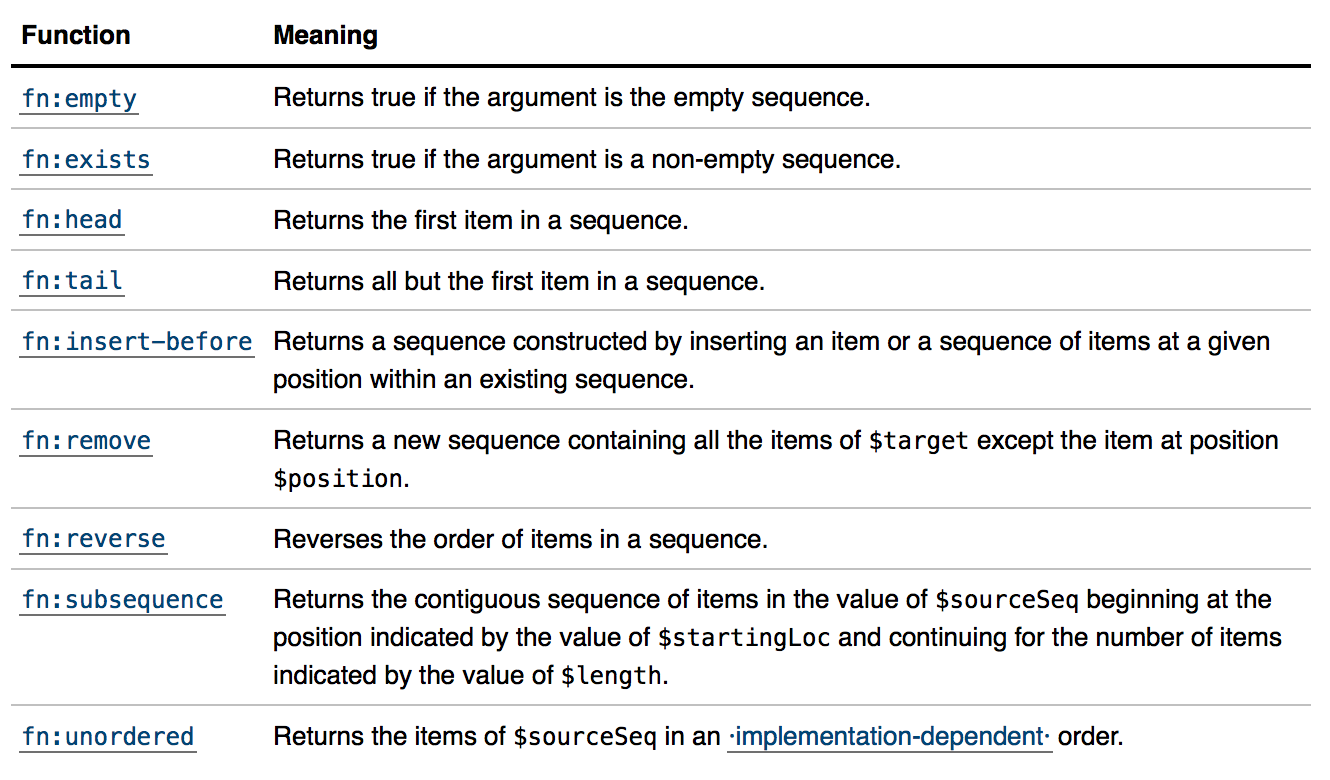
\includegraphics[width=\textwidth]{figures/XQuery_sequence_functions1.png}

\end{frame}

\begin{frame}[fragile]
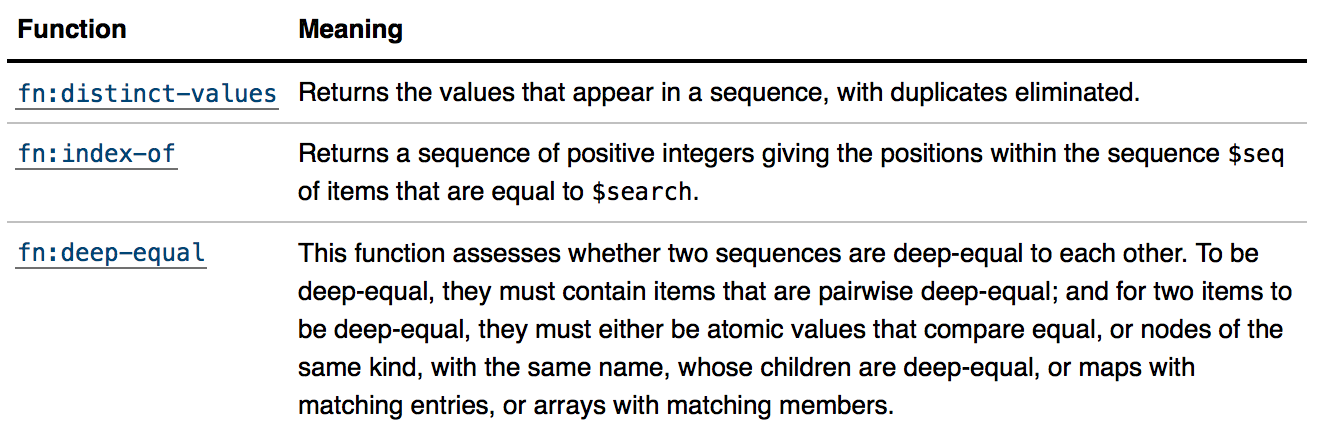
\includegraphics[width=\textwidth]{figures/XQuery_sequence_functions2.png}

Example:

\begin{lstlisting}[style=XQuery]
for -:$n:- in distinct-values(doc("books.xml")//publisher/text())
return <publisher>{-:$n:-}</publisher>
\end{lstlisting}

\begin{onlyenv}<2-| handouts:1>
\begin{lstlisting}[style=markup]
<publisher>Cambridge</publisher><publisher>MIT Press</publisher>
\end{lstlisting}

\vskip1em

Why do we \textbf{need} \lstinline[style=XQuery]!text()! in the path expression above?
\end{onlyenv}
\end{frame}


\begin{frame}[fragile]
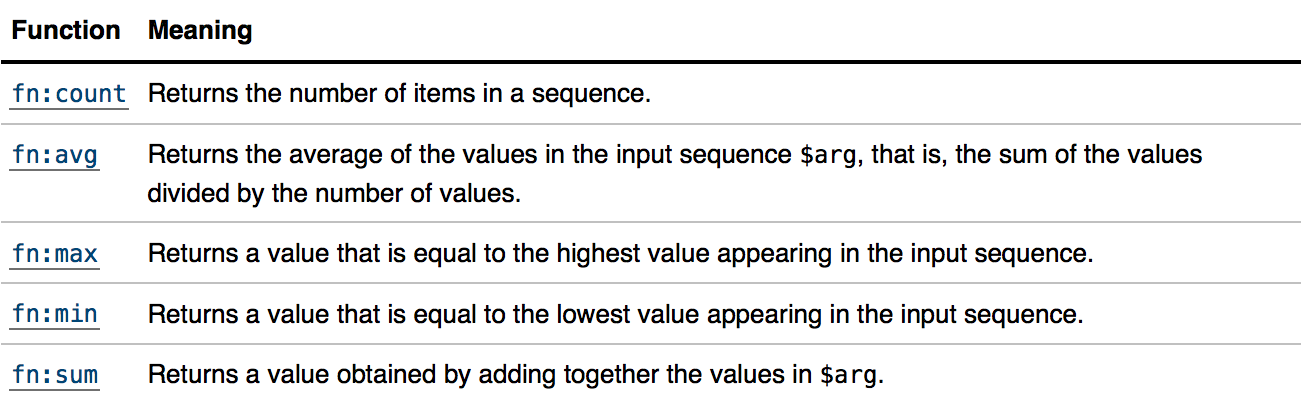
\includegraphics[width=\textwidth]{figures/XQuery_sequence_functions3.png}

Example:

\begin{lstlisting}[style=XQuery]
let -:$cnts:- := for $b in doc("books.xml")//book
             return count($b/author)
return round(avg(-:$cnts:-), 2)
\end{lstlisting}

\begin{onlyenv}<2-| handouts:1>
\begin{lstlisting}[style=markup]
2
\end{lstlisting}
\end{onlyenv}
\end{frame}

\begin{frame}[fragile]{Comparisons Involving Sequences}

Recall the \alert{general comparators} that apply to values and sequences:

\begin{itemize}[noitemsep]
\item \lstinline[style=XQuery]!-:=:-! (equals to) \qquad\qquad\qquad \lstinline[style=XQuery]{-:!=:-} (different than)
\item \lstinline[style=XQuery]!-:<:-! (less than) \qquad\qquad\qquad \lstinline[style=XQuery]!-:<=:-! (less than or equal to)
\item \lstinline[style=XQuery]!-:>:-! (greater than) \qquad\qquad~~ \lstinline[style=XQuery]!-:>=:-! (greater than or equal to)
\end{itemize}

\vskip1em

\begin{block}{Existential Semantics}
\lstinline[style=XQuery]!$s1  OP $s2! evaluates to \textbf{true} if \underline{there exist} items \alert{\texttt{x}} in \lstinline[style=XQuery]!$s1! and \alert{\texttt{y}} in \lstinline[style=XQuery]!$s2! for which \lstinline[style=XQuery]!x OP y! is true.
\end{block}

Examples: all programs below return \textbf{true}...

\begin{columns}[onlytextwidth]
\begin{column}{0.3\textwidth}
\begin{lstlisting}[style=XQuery]
let $s1 := (1,2,3)
let $s2 := (1,2)
return $s1 = $s2
\end{lstlisting}
\end{column}

\begin{column}{0.3\textwidth}
\begin{lstlisting}[style=XQuery]
let $s1 := (1,2,3)
let $s2 := (1,2)
return $s1 @< $s2
\end{lstlisting}
\end{column}

\begin{column}{0.3\textwidth}
\begin{lstlisting}[style=XQuery]
let $s1 := (1,2,3)
let $s2 := (1,2)
return $s1 > $s2
\end{lstlisting}
\end{column}
\end{columns}
\end{frame}


\begin{frame}[fragile]
\textbf{\blue{Comparisons with sequences can be convenient...}}

\vskip0.5em

\textbf{Ex:} find the titles of books that have at least one author whose first name is Prabhakar

\begin{lstlisting}[style=XQuery]
for $b in doc("books.xml")//book
where $b/author/first/text() = "Prabhakar"
return $b/title
\end{lstlisting}

Returns

\begin{lstlisting}[style=XQuery]
<title>Introduction to Information Retrieval</title>
\end{lstlisting}

\vskip1em

Why? For that book, we have that \\ \lstinline[style=XQuery]!$b/author/first/text()! $\leftarrow$ \lstinline[style=XQuery]!("Christopher", "Prabhakar", "Hinrich")!.

\end{frame}


\begin{frame}[fragile]

XQuery uses \alert{casting} aggressively, in an attempt to simplify the queries. The following expression from the previous query compares two \textbf{sequences}:

\begin{center}
\lstinline[style=XQuery]!$b/author/first/text() = "Prabhakar"!
\end{center}

% \vskip1em

XQuery casts the RHS to \lstinline[style=XQuery]!( "Prabhakar" )!

The following query (note it does not have \lstinline[style=XQuery]!text()!) computes the same answer:

\begin{lstlisting}[style=XQuery]
for $b in doc("books.xml")//book
where $b/author/first = "Prabhakar"
return $b/title
\end{lstlisting}

XQuery understands the RHS is a sequence of values, and casts each \lstinline[style=XQuery]!<first>! element into the corresponding value.

\end{frame}


\begin{frame}[fragile]
\textbf{\blue{But comparisons with sequences can also be confusing...}}

\textbf{Ex:} find the titles of books that have at least one author whose first name is Prabhakar and last name is Manning. 

\begin{lstlisting}[style=XQuery]
for $b in doc("books.xml")//book
where $b/author/first = "Prabhakar" and $b/author/last = "Manning"
return $b/title
\end{lstlisting}

The query ``should return nothing'' (as there is no author satisfying the conditions). Yet, it returns:

\begin{lstlisting}[style=XQuery]
<title>Introduction to Information Retrieval</title>
\end{lstlisting}

\vskip1em

Why? For that book, both \\\lstinline[style=XQuery]!("Christopher", "Prabhakar", "Hinrich") = "Prabhakar"! and \\ \lstinline[style=XQuery]!("Manning", "Raghavan", "Schütze") = "Manning"! evaluate to true.

\end{frame}


\begin{frame}[fragile]
Fixing the query so that it finds correctly the titles of books that have at least \emph{one author} whose first name is Prabhakar and last name is Manning.

\begin{lstlisting}[style=XQuery]
for $b in doc("books.xml")//book
where $b/author/first = "Prabhakar" and $b/author/last = "Manning"
return $b/title
\end{lstlisting}

\vskip1em 

\begin{onlyenv}<2-| handouts:1>
\begin{lstlisting}[style=XQuery]
for $b in doc("books.xml")//book
  for $a in $b/author
  where $a/first = "Prabhakar" and $a/last = "Manning"
  return $b/title

\end{lstlisting}
\end{onlyenv}

\end{frame}



\begin{frame}[fragile]{Nested Loops}

\begin{columns}[onlytextwidth]
\begin{column}{0.4\textwidth}

The previous query is an example of a \emph{correlated} nested loop:

\vskip2em

\begin{lstlisting}[style=XQuery]
for $b in doc("books.xml")//book
   for $a in $b/author
      return $a/last
\end{lstlisting}

\vskip1em

\begin{onlyenv}<2-| handouts:1>
\begin{lstlisting}[style=markup]
<last>Pearl</last>
<last>Manning</last>
<last>Schütze</last>
<last>Manning</last>
<last>Raghavan</last>
<last>Schütze</last>
\end{lstlisting}
\end{onlyenv}
\end{column}

\begin{column}{0.5\textwidth}
\scalebox{0.75}{\clipbox{0pt -1pt 3em 0.5em}{\scalebox{0.75}{\usebox\biblioXML}}}
\end{column}

\end{columns}
\end{frame}

\begin{frame}[fragile]{Products and Joins}

We write cross products explicitly as nested loops:

\begin{columns}
\begin{column}{0.5\textwidth}
\begin{lstlisting}[style=XQuery]
let $s1 := (1,2,3)
let $s2 := (1,2)
for $a in $s1
  for $b in $s2
  return <pair>{ $a , ":" , $b }</pair>
\end{lstlisting}
\end{column}
\begin{column}{0.25\textwidth}
\begin{lstlisting}[style=XQuery]
<pair>1 : 1</pair>
<pair>1 : 2</pair>
<pair>2 : 1</pair>
<pair>2 : 2</pair>
<pair>3 : 1</pair>
<pair>3 : 2</pair>
\end{lstlisting}
\end{column}
\end{columns}

\vskip1em

Recall a join is a cross product followed by a selection...

\begin{columns}
\begin{column}{0.5\textwidth}
\begin{lstlisting}[style=XQuery]
let $s1 := (1,2,3)
let $s2 := (1,2)
for $a in $s1
  for $b in $s2
  where $a eq $b
  return <pair>{ $a , ":" , $b }</pair>
\end{lstlisting}
\end{column}
\begin{column}{0.25\textwidth}
\begin{lstlisting}[style=XQuery]
<pair>1 : 1</pair>
<pair>2 : 2</pair>
\end{lstlisting}
\end{column}
\end{columns}
\end{frame}

\begin{frame}[fragile]{More Joins}

Suppose we have two XML files: \lstinline!books.xml! as before and \lstinline!loans.xml! to keep track of books loaned out to library users.

The following query joins the two files, returning the titles of the books which are loaned and due (at the date the query executes).

\vskip1em

\begin{lstlisting}[style=XQuery]
let $due := for $h in doc("holdings.xml")//loan
  where $h/due eq current-date()
  return $h
for $b in doc("books.xml")//book
   for $h in $due
   where $h/@isbn eq $b/@isbn
   return $b/title
\end{lstlisting}

\end{frame}


\begin{frame}[fragile]{Aggregation in XQuery 1.0}

XQuery V1.0 does not have an explicit clause for aggregation, unlike SQL. Aggregation can still be accomplished through nested loops.

\textbf{Example:} counting the books per publisher.

\begin{lstlisting}[style=XQuery]
let $publishers := distinct-values(doc("books.xml")//publisher/text())
for $p in $publishers
  let $books := doc("books.xml")//book[./publisher/text() eq $p ]
  return <book_counts><publisher>{$p}</publisher>
                      <count>{count($books)}</count>
         </book_counts>
\end{lstlisting}


\vskip1em

However, developers missed the familiar construct from SQL. 

From an implementation point of view, having an explicit clause for aggregation would allow XQuery implementers to optimize that operation as well.

\end{frame}


\newsavebox{\aggregationXQueryTWO}
\begin{lrbox}{\aggregationXQueryTWO}
\begin{lstlisting}[style=XQuery]
for $b in doc("books.xml")//book
let $p := $b/publisher
group by $p
return  <book_counts>
          <publisher>{$p}</publisher>
          <count>
            {count($b)}
          </count>
         </book_counts>
\end{lstlisting}
\end{lrbox}

\newsavebox{\resultEXTWO}
\begin{lrbox}{\resultEXTWO}
\begin{lstlisting}[style=markup]
<book_counts>
  <publisher>Cambridge</publisher>
  <count>2</count>
</book_counts>
<book_counts>
  <publisher>MIT Press</publisher>
  <count>1</count>
</book_counts>
\end{lstlisting}
\end{lrbox}

\begin{frame}[fragile]{Aggregation in XQuery 1.1}

XQuery 1.1 brought new features, many of which were familiar to SQL developers, including an \lstinline[style=XQuery]!group by! clause.

\textbf{Example:} counting the books per publisher.`'

\begin{columns}[onlytextwidth]
\begin{column}{0.5\textwidth}
\scalebox{0.95}{\usebox{\aggregationXQueryTWO}}
\end{column}
\begin{column}{0.45\textwidth}
\scalebox{0.8}{\usebox{\resultEXTWO}}
\end{column}
\end{columns}

\vskip1em

Multiple attributes and multiple \emph{sequence} functions can be used in the aggregation.

\end{frame}

\begin{frame}[fragile]

\vskip1em

\textbf{\alert{Warning}:} there must be a 1-1 relationship between the elements being aggregated and the elements defining the groups!

\vskip1em

\begin{columns}[onlytextwidth]
\begin{column}{0.45\textwidth}
This works because each book has a single publisher (i.e., a single group).

\vskip1em

If there were multiple \lstinline[style=XQuery]!$p! for a single \lstinline[style=XQuery]!$b! you would have to ``un-nest'' those pairs first:
\end{column}
\begin{column}{0.5\textwidth}
\scalebox{0.9}{\usebox{\aggregationXQueryTWO}}
\end{column}
\end{columns}

\vskip0.5em

\begin{lstlisting}[style=XQuery]
let $pairs := for $b in doc("books.xml")//book
              for $p in $b/publisher
              return <pair>{$b,$p}</pair>
for $pair in $pairs
let $p := $pair/publisher
group by $p
...
\end{lstlisting}


\end{frame}


\begin{frame}[fragile]{Order By}

The \lstinline[style=XQuery]!order by! clause sorts elements in a sequence.

\vskip1em

Example

\begin{lstlisting}[style=XQuery]
let $lnames := distinct-values(doc("books.xml")//author/last/text())
for $n in $lnames
order by $n ascending
return <name>{ $n }</name>
\end{lstlisting}

\vskip1em

Returns
\begin{onlyenv}<2-| handouts:1>
\begin{lstlisting}[style=markup]
<name>Manning</name>
<name>Pearl</name>
<name>Raghavan</name>
<name>Schütze</name>
\end{lstlisting}
\end{onlyenv}
\end{frame}


\begin{frame}[fragile]{Type Conversion}

Unless otherwise specified by an XML Schema, the content of every element and/or attribute in a document is of type \alert{string}.

Like with SQL, we can cast string types to numbers\footnote{\url{https://www.w3.org/TR/xpath-functions-31/\#casting-to-numerics}}:

\vskip1em

\begin{lstlisting}[style=XQuery]
for $b in doc("books.xml")//book
where xs:integer($b/@year) gt 2000
return $b
\end{lstlisting}

\vskip1em

In fact, XQuery has a complex and rich type system.

\end{frame}


\begin{frame}[fragile]{Quantification in XQuery}

XQuery designers made explicit existential and universal quantification part of the language. 

\vskip2em

\alert{Existential quantification is the \textbf{default}}, so the two queries below are equivalent.

\begin{lstlisting}[style=XQuery]
for $b in doc("books.xml")//book
where $b/author/first = "Prabhakar"
return $b/title
\end{lstlisting}


\begin{lstlisting}[style=XQuery]
for $b in doc("books.xml")//book
where some $f in $b/author/first satisfies ($f eq "Prabhakar")
return $b/title
\end{lstlisting}

\end{frame}

\begin{frame}[fragile]{Quantification in XQuery}
\alert{Universal quantification} is also written explicitly:

Ex: which publishers have published all books by Christopher Manning?

\begin{lstlisting}[style=XQuery]
let $books := doc("books.xml")//book
let $CMbooks := for $b in $books
                where some $a in $b/author satisfies
                    ($a/first/text() eq "Christopher" and 
                     $a/last/text() eq "Manning")
                return $b

for $p in $books/publisher/text()
where every $CMpublisher in $CMbooks/publisher satisfies
  $p = $CMpublisher
return $p
\end{lstlisting}
\end{frame}

\begin{frame}[fragile]

Ex: Which authors co-wrote all books with Christopher Manning?

\begin{lstlisting}[style=XQuery]
let $books := doc("books.xml")//book
let $CMbooks := for $b in $books
                where some $a in $b/author satisfies
                    ($a/first/text() eq "Christopher" and 
                     $a/last/text() eq "Manning")
                return $b

for $a in $CMbooks/author
where every $b in $CMbooks satisfies
  some -:$coauthor:- in $b/author satisfies $a = -:$coauthor:-
return $a
\end{lstlisting}

\end{frame}

\begin{frame}{What else?}

A \textbf{lot} more...

\begin{itemize}[-]
\item \alert{User-defined functions}. XQuery is a fully functional language, and allows users to define their own functions in XQuery itself.

\item \alert{Recursion}. XQuery allows recursive function calls, in a way that is familiar to all programmers.

\item Familiar \alert{programming constructs} (e.g., \lstinline[style=XQuery]{if-then-else}). 

\item A very rich \alert{standard library}, sufficient for a wide range of applications.

\item Support for \alert{updates} to documents.
\end{itemize}

XQuery is powerful enough to implement virtually anything that a Web service provider might need.

\end{frame}











\section{XML Support in DBMSs}
%!TEX root = lec07_documents.tex

\begin{frame}{Approaches for storing XML}

\begin{itemize}[-]
\item File System: keep documents as text files.
\item Native XML Store.
\begin{itemize}[-]
\item Implement persistent data structures to represent the XML (DOM) tree.
\end{itemize}
\item Inside a Relational DBMS: re-use existing storage, indexing, (and querying) systems.
\begin{itemize}[-]
\item String or BLOB attribute.
\item \emph{XML Mappings}.
\begin{itemize}[$\star$]
\item Schema-based.
\item Structure-based.
\end{itemize}
\end{itemize}
\end{itemize}
\end{frame}


\begin{frame}{XML documents in the File System}

\begin{itemize}[-]
\item Advantages:
\begin{itemize}[-]
\item Simplicity. 
\item Re-using existing I/O layer (and file-level locking) provided by the Operating System.
\end{itemize}

\item Disadvantages:
\begin{itemize}[-]
\item Document (and data therein) is exposed to \alert{any user} and/or \alert{any tool} (e.g., a text editor) that has access to the directory where the documents are stored.
\item Duplicated efforts: logging, concurrency control, back-ups, security, etc. are done outside the DBMSs.
\item Hard to coordinate queries that involve relational (in-DBMS) and XML (out-of-DBMS) data.
\end{itemize}
\end{itemize}
\end{frame}

\begin{frame}{Native XML Stores}

These systems are tailored for working with XML documents of any size (typically, they support up to a few GB per document), supporting queries and update natively.

In a sense, these are highly I/O optimized implementations of tree data-structures.

Some systems listed on Wikipedia (circa 2019):

\hspace*{-20pt}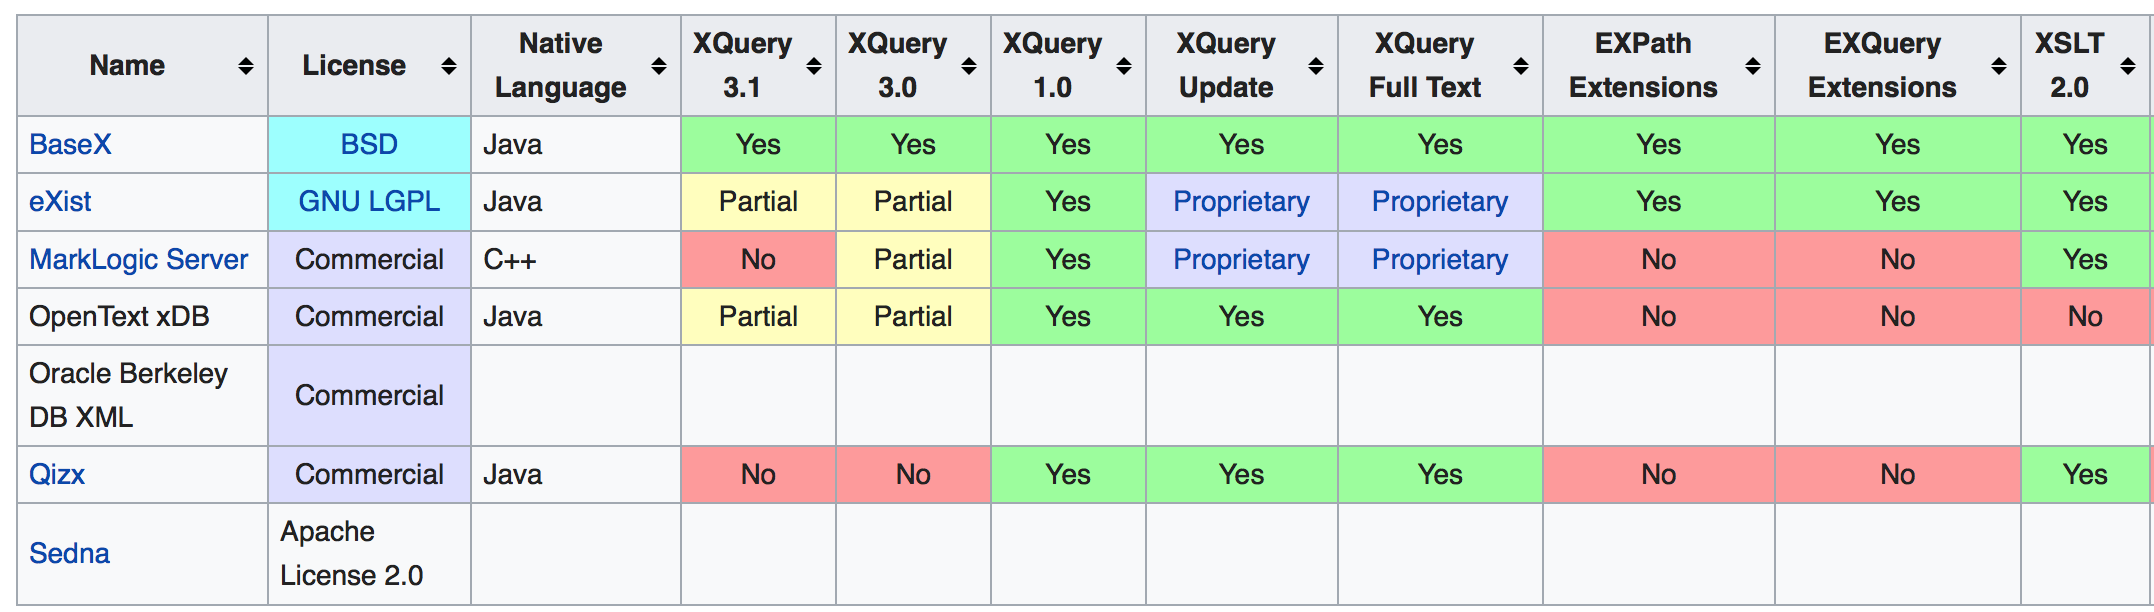
\includegraphics[width=1.15\textwidth]{figures/native_XML_stores.png}
\end{frame}


\begin{frame}{Native XML Stores}

Full fledged native stores combine the functionality of a file server (e.g., WebDAV support) and a Web server (HTTP support) with that of a database management system (e.g., command-line SQL and API support for queries and updates, indexing, transaction management, etc.).

For commercial reasons, XML Stores must also support SQL systems to be successful. 

Some strategies:
\begin{itemize}[-]
\item Exporting XML data as relational views that can be read and modified by an external application.
\item Offering native SQL support.
\end{itemize}
\end{frame}

\begin{frame}{Oracle XML DB}
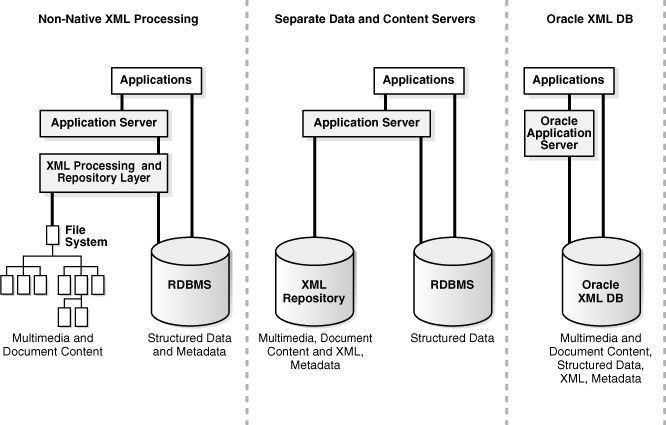
\includegraphics[width=\textwidth]{figures/Oracle_XMLDB.png}

\footnotesize Source \url{https://docs.oracle.com/cd/B19306_01/appdev.102/b14259/xdb01int.htm}
\end{frame}


\begin{frame}
\begin{center}
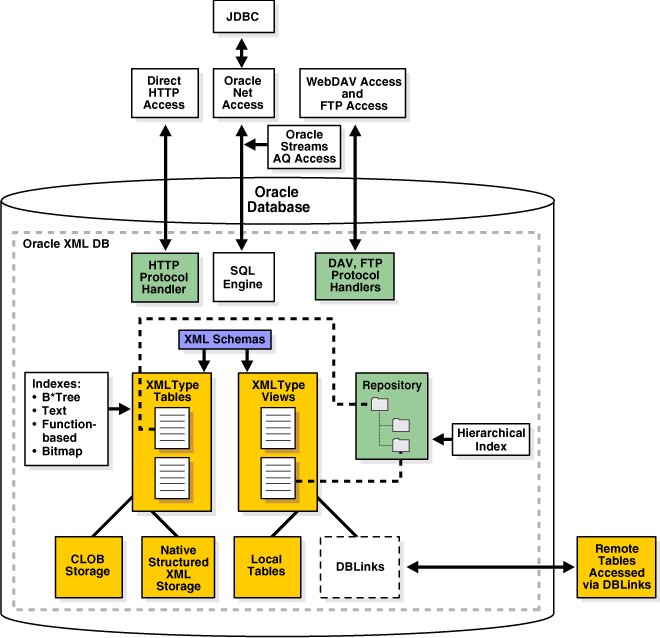
\includegraphics[width=0.75\textwidth]{figures/Oracle_XMLDB2.png}
\end{center}
\footnotesize Source \url{https://docs.oracle.com/cd/B19306_01/appdev.102/b14259/xdb01int.htm}
\end{frame}

\begin{frame}{BaseX}

BaseX was started by Christian Grün at the University of Konstanz in 2005. In 2007, BaseX went open source and has been BSD-licensed since then.

Fully developed in Java.

Supports XPath, XQuery 3.1, WebDAV, and various API/connector protocols.

Concurrency control:
\begin{itemize}[-]
\item Queries run in parallel.
\item Updates run with locking.
\end{itemize}

\footnotesize Sources \url{http://basex.org} and \url{https://en.wikipedia.org/wiki/BaseX}
\end{frame}

\begin{frame}{eXist}

eXist is an open-source \alert{client/server} native XML database manager supporting all popular XML protocols, XQuery, indexing, updates, proper concurrency control, \textbf{triggers}, and more!

\vskip2em

\begin{center}
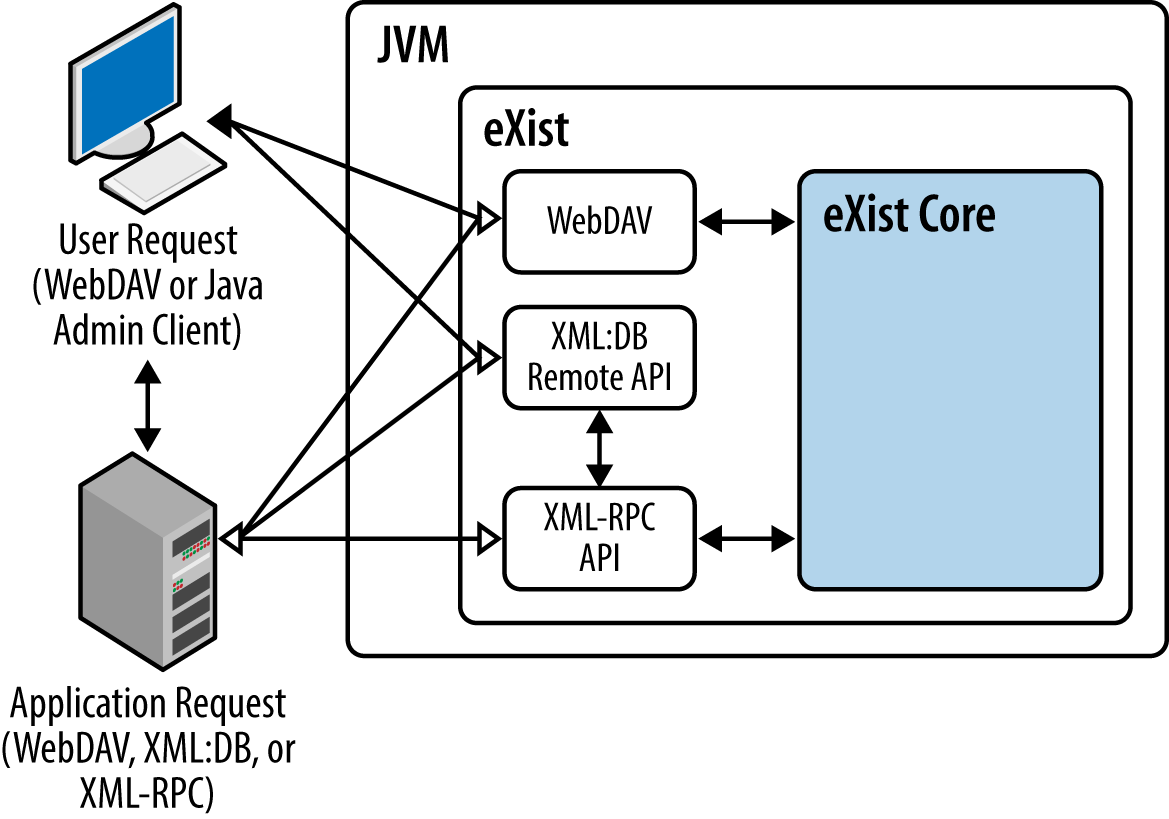
\includegraphics[width=0.6\textwidth]{figures/eXist_clientServer.png}
\end{center}

\footnotesize Source: eXist, by Retter and Siegel, O'Reilly 2014\\\url{https://learning.oreilly.com/library/view/exist/9781449337094/}
\end{frame}

\begin{frame}
\vskip1em
\begin{columns}[onlytextwidth]
\begin{column}{0.25\textwidth}

\footnotesize Source: eXist, by Retter and Siegel, O'Reilly 2014

\end{column}
\begin{column}{0.6\textwidth}
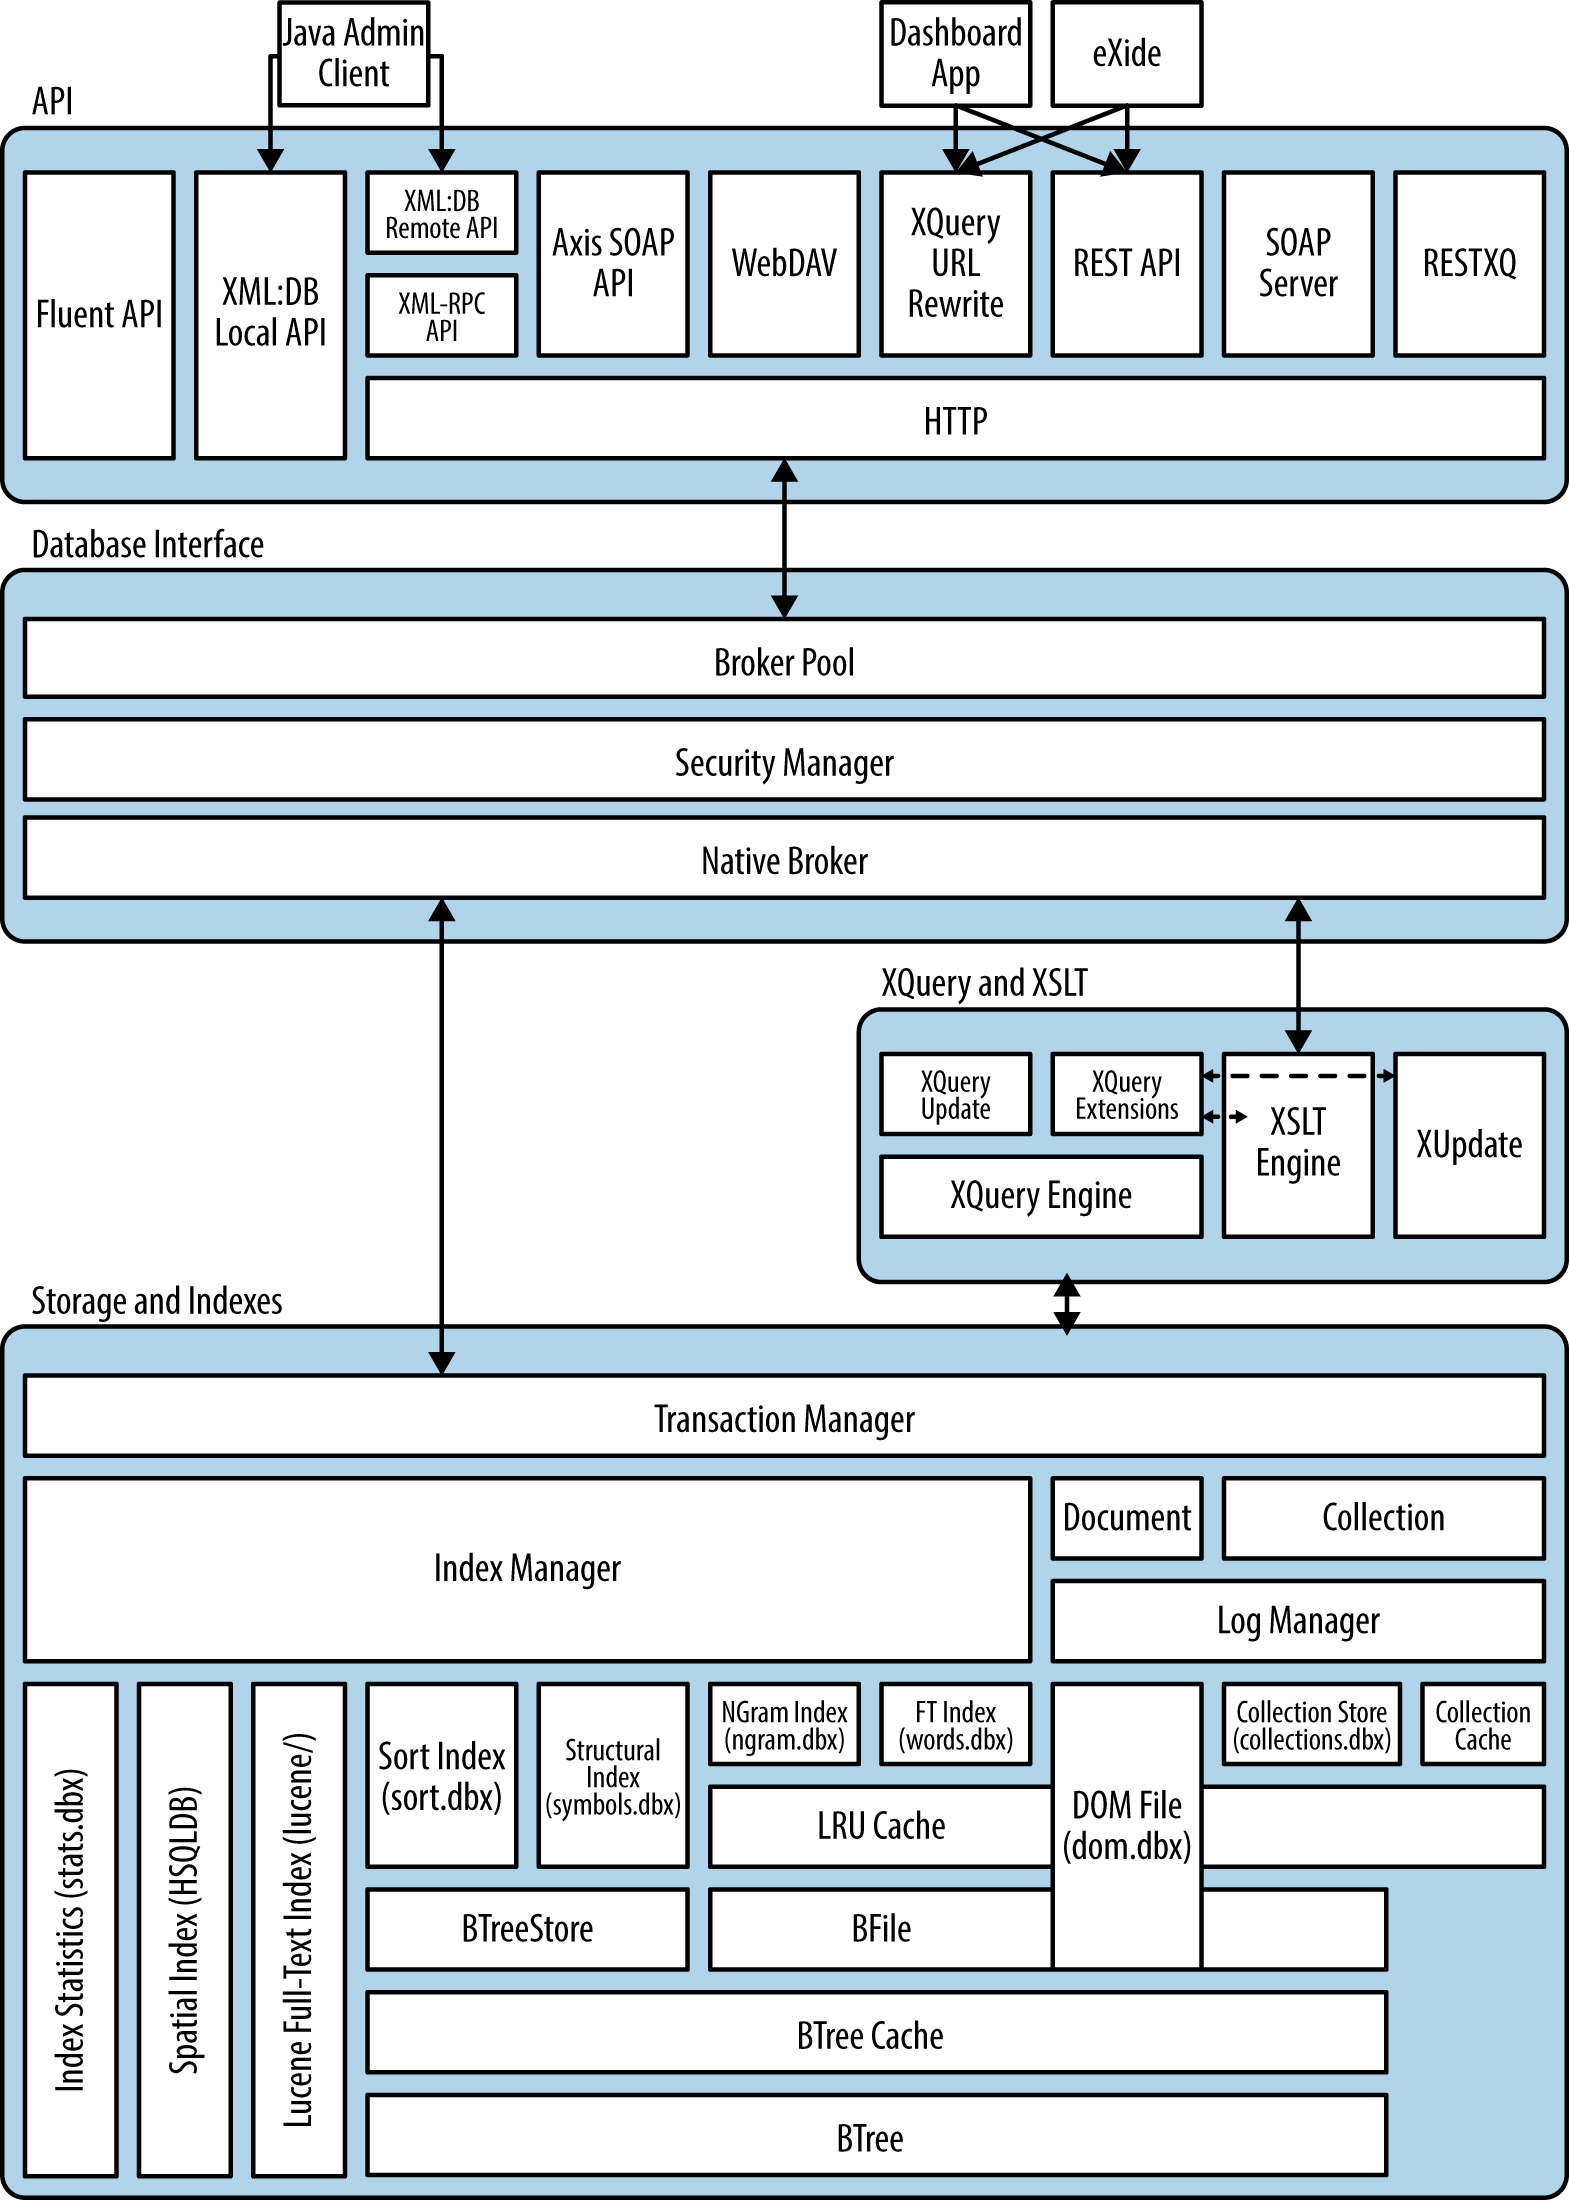
\includegraphics[width=1\textwidth]{figures/eXist_architecture.png}
\end{column}
\end{columns}
\end{frame}


\begin{frame}{Native XML Stores}

Native XML stores are a form of NoSQL that has gained much popularity since the mid-2000s, and can be used in support of document stores and Web Services.

\begin{itemize}[-]
\item Advantages:
\begin{itemize}[-]
\item Can implement optimizations specific for XML and XQuery.
\item Single application development platform.
\item ``Single Source of Truth'' for XML data: avoid fragmenting or mapping data into possibly inconsistent pieces.
\end{itemize}
\item Disadvantages:
\begin{itemize}[-]
\item Might not integrate well with existing legacy applications.
\end{itemize}
\end{itemize}
\end{frame}


\begin{frame}{RDBMS support for XML}

With the rise of native XML database management systems, many applications were ported away from RDBMSs. 

Relational vendors responded by offering support for XML within their relational products, which came in two forms: 

\begin{itemize}[-]
\item An \alert{XML data type} which can be used to store (\alert{native}ly) XML documents as attributes of a regular tuple.
\item \alert{XML Mappings}, in which XML data and queries are \alert{translated} into relational data and queries.
\end{itemize}

An industry standard, SQL/XML\footnote{\url{https://en.wikipedia.org/wiki/SQL/XML}} was defined with extensions to relational systems to handle XML content and queries.

\end{frame}


\begin{frame}[fragile]{XML Data Type}

With this approach, XML content is stored as \alert{an attribute of a tuple} with the XML data type. 

Example from the IBM DB2 documentation:

\vskip1em

\bgroup
\begin{lstlisting}[style=SQL,emph={XML},emphstyle=\color{red}]
CREATE TABLE Customer (Cid BIGINT NOT NULL PRIMARY KEY,
                       Info XML,
                       History XML)
\end{lstlisting}
\egroup

SQL is still used as the main language for querying the database, and for inserting and modifying data.

To manipulate the XML content, we use either custom SQL functions that XPath/XQuery or SQL/XML extensions.

\end{frame}


\begin{frame}[fragile]{Inserting XML Content}

Special API calls are used to insert XML content.

Example from the IBM DB2 documentation:


\vskip1em

\bgroup

\lstset{
    style=cmput391,
	language=Java,
	basicstyle=\ttfamily\scriptsize,
	commentstyle=\color{fern},
	stringstyle=\color{stringColor},
	keywordstyle=\color{functionColor},
	keywords=[1]{conn,insertStmt},
	emphstyle=[1]\color{blue},
	emph=[1]{prepareStatement,File,setBinaryStream,executeUpdate}
}

\begin{lstlisting}
PreparedStatement insertStmt = null; 

int cid = 12345; // some customer id
String sqls = "INSERT INTO Customer (Cid, Info) VALUES (?, ?)";

java.sql.Connection conn = ... //initialize connection

insertStmt = conn.prepareStatement(sqls);
insertStmt.setInt(1, cid);

File file = new File("c6.xml");

insertStmt.setBinaryStream(2, new FileInputStream(file), (int)file.length());
insertStmt.executeUpdate();
\end{lstlisting}

\egroup
\end{frame}


\newsavebox\XMLAGGphoneListExample
\begin{lrbox}{\XMLAGGphoneListExample}
\begin{lstlisting}[style=markup,basicstyle=\ttfamily\scriptsize]
<customerinfo Cid="12345">
  <name>Kathy Smith</name>
  <addr country="Canada">
    <street>5 Rosewood</street>
    <city>Toronto</city>
    <prov-state>Ontario</prov-state>
    <pcode-zip>M6W 1E6</pcode-zip>
  </addr>
  <phone type="work">416-555-1358</phone>
</customerinfo>
\end{lstlisting}
\end{lrbox}


\begin{frame}[fragile]{Querying XML Data in an XML Column}

\vskip1em

\begin{columns}[onlytextwidth]
\begin{column}{0.55\textwidth}


Example from the IBM DB2 documentation:

\vskip0.5em

Suppose the XML document to the right is inserted into the \lstinline[basicstyle=\ttfamily\small\color{blue}]!INFO! attribute of some tuple.

\end{column}
\begin{column}{0.5\textwidth}
\scalebox{0.8}{\usebox{\XMLAGGphoneListExample}}
\end{column}
\end{columns}

\vskip0.5em

We can query that document by invoking XQuery via an SQL extension:

\bgroup

\begin{lstlisting}[style=SQL,basicstyle=\ttfamily\scriptsize]
SELECT -:XMLQUERY:- ("document{<phonelist>{$doc/customerinfo/phone}</phonelist>}"
  -:PASSING:- INFO AS "doc")
FROM CUSTOMER
WHERE Cid=12345
\end{lstlisting}
\egroup

\vskip-0.5em
Result: \lstinline[style=markup]!<phonelist><phone type="work">416-555-1358</phone></phonelist>!

\end{frame}


\newsavebox\movieCastSQLXML
\begin{lrbox}{\movieCastSQLXML}
\begin{lstlisting}[style=SQL]
SELECT -:XMLelement:-(-:NAME:- "Movies",
        -:XMLAGG:-(
          -:XMLelement:- (-:NAME:- "movie",
            -:XMLelement:- (-:NAME:- "title", m.title),
            -:XMLelement:- (-:NAME:- "year", m.year),
            -:XMLelement:- (-:NAME:- "cast",
              (SELECT -:XMLAGG:-(
                -:XMLelement:-(-:NAME:- "actor", 
                   -:XMLattributes:-(c.role AS "role"), c.actor))
               FROM movies.Cast c 
               WHERE c.title=m.title and c.year=m.year)
              ) -- cast element 
          ) -- movie element
        ) -- XMLAGG
      ) -- Movies element
FROM movies.Movie m
WHERE EXISTS(
  SELECT * 
  FROM movies.Cast
  WHERE actor = 'Bill Murray' AND title=m.title AND year=m.year
);
\end{lstlisting}
\end{lrbox}

\begin{frame}[fragile]{Exporting relational data as XML}

 PostgreSQL SQL/XML (on the movies database):

\begin{center}
\scalebox{0.75}{\usebox{\movieCastSQLXML}}
\end{center}
\end{frame}

\newsavebox\movieCastXMLdump
\begin{lrbox}{\movieCastXMLdump}
\begin{lstlisting}[style=markup]
<Movies>
    <movie>
        <title>Lost in Translation </title>
        <year>2003</year>
        <cast>
            <actor role="Bob Harris">Bill Murray </actor>
        </cast>
    </movie>
    <movie>
        <title>Ghostbusters </title>
        <year>1984</year>
        <cast>
            <actor role="Dr. Venkman">Bill Murray </actor>
            <actor role="Dana Barret">Sigourney Weaver </actor>
        </cast>
    </movie>
</Movies>
\end{lstlisting}
\end{lrbox}

\begin{frame}[fragile]

Result:

\begin{center}
\scalebox{0.75}{\usebox{\movieCastXMLdump}}
\end{center}

\end{frame}


% \begin{frame}[fragile]
% Another example (tested on IBM DB2 and Oracle):

% \bgroup

% \lstset{
%     style=cmput391,
% 	basicstyle=\ttfamily\scriptsize,
% 	morecomment=[l]{--},
% 	commentstyle=\color{fern},
% 	stringstyle=\color{stringColor},
% 	keywordstyle=\color{functionColor},
% 	keywords=[1]{XMLQUERY,XMLELEMENT,XMLATTRIBUTE,XMLAGG,PASSING},
% 	emphstyle=[1]\color{blue},
% 	emph=[1]{doc,INFO}
% }

% \begin{lstlisting}[style=SQL]
% SELECT -:XMLELEMENT:-(NAME "PhoneBook", -- root element name
%           -:XMLAGG:-(           -- aggregation over the rows
%               -:XMLELEMENT:-(NAME "Contact",                                                  
%                  -:XMLATTRIBUTE:-(cust.FIRST_NAME AS "Name",
%                                  cust.TEL)
%                  )
%               )
%       )
% FROM CUSTOMER AS cust;
% \end{lstlisting}

% Result:

% \begin{lstlisting}[style=markup,basicstyle=\ttfamily\scriptsize]
% <PhoneBook>
%     <Contact Name="Daniel" TEL="788255855"/>
%     <Contact Name="Martin" TEL="889665447"/>
%     <Contact Name="Eva"    TEL="111222333"/>
%     <Contact Name="Alena"  TEL="444555666"/>
%     <Contact Name="Oliver" TEL="777888999"/>
%     <Contact Name="George" TEL="444882446"/>
%     <Contact Name="Jamie"  TEL="123456789"/>
% </PhoneBook>
% \end{lstlisting}

% \egroup

% \end{frame}

\begin{frame}{SQL/XML: summary}

\begin{itemize}[-]
\item Advantages:
\begin{itemize}[-]
\item Industry standard supported by many vendors and likely to remain relevant for industry.
\item Single interface for querying relational and XML data.
\item Very practical for \alert{exporting relational data as XML}.
\end{itemize}
\item Disadvantages:
\begin{itemize}[-]
\item Fairly complex standard. 
\item XQuery and SQL are not fully compatible. 
\item Very hard to optimize.
\end{itemize}
\end{itemize}

\end{frame}


\begin{frame}{Storing XML via Mappings}

The main motivation behind developing XML mappings was to leverage existing and highly optimized relational machinery instead of developing everything new again, for XML.

(Recall that XML documents are trees, and that we can represent arbitrary graphs (including trees) inside a relational database.)

\vskip1em

\begin{block}{mapping = translation}
With this approach, we:
\begin{itemize}[-]
\item \alert{Translate} XML data into \textbf{pure relational data}.
\item \alert{Translate} XQuery queries into \textbf{pure SQL}.
\end{itemize}
\end{block}

There are two kinds of mappings: based on the tree structure of the data, and based on the tags.
\end{frame}

\begin{frame}{Semantic Mappings}

Semantic Mappings are intended for the cases when XML data comes with a schema (or DTD). The idea is to use \alert{``mapping patterns''} to handle common constructs in a schema (or DTD).

\vskip1em

Examples:

\begin{block}{Pattern {\textcolor{red}{\textsf{a (..., b*, ...)}}}}
\begin{enumerate}[(1),noitemsep]
\item Use separate tables for {\textcolor{red}{\textsf{a}}} and {\textcolor{red}{\textsf{b}}}.
\item Define a foreign key from {\textcolor{red}{\textsf{b.id}}} into {\textcolor{red}{\textsf{a.id}}}.
\end{enumerate}
\end{block}

\begin{block}{Pattern {\textcolor{red}{\textsf{a (..., b+, ...)}}}}
\begin{enumerate}[(1),noitemsep]
\item Do as in the Pattern {\textcolor{red}{\textsf{a (b*)}}}.
\item Define trigger to make sure a {\textcolor{red}{\textsf{b}}} is always present for every {\textcolor{red}{\textsf{a}}}.
\end{enumerate}
\end{block}
\end{frame}

\begin{frame}[fragile]

\begin{block}{Pattern {\textcolor{red}{\textsf{a (..., b?, ...)}}}}
\begin{enumerate}[(1),noitemsep]
\item Add an attribute {\textcolor{red}{\textsf{b}}} to the table for {\textcolor{red}{\textsf{a}}}.
\end{enumerate}
\end{block}

\begin{block}{Pattern {\textcolor{red}{\textsf{a (..., b, ...)}}}}
\begin{enumerate}[(1),noitemsep]
\item Add an attribute {\textcolor{red}{\textsf{b}}} to the table for {\textcolor{red}{\textsf{a}}}.
\item Define the attribute to be \textbf{required} (i.e., \lstinline[style=SQL]!NOT NULL!).
\end{enumerate}
\end{block}

\vskip1em

Dealing with XML attributes can be done in a similar way (i.e., they become ``SQL attributes'' of the table that stores the corresponding XML element).
\end{frame}

\begin{frame}[fragile]{Database Constraints}

To enforce the restrictions on \lstinline[language=DTD]!-:#ID:-! and \lstinline[language=DTD]!-:#IDREF:-! attributes, we need to use \textbf{triggers}:

\begin{itemize}[-,topsep=-5pt]
\item \alert{\textbf{Before} inserting} a tuple with an \lstinline[language=DTD]!-:#ID:-! attribute, check that no other such attribute (in any of the tables with such attributes) has the same value as the one in the \lstinline[style=SQL]!new! tuple.
\item \alert{\textbf{Before} inserting} a tuple with an \lstinline[language=DTD]!-:#IDREF:-! attribute, check that the value in the \lstinline[style=SQL]!new! tuple exists in the database (in any of the tables with \lstinline[language=DTD]!-:#ID:-! attributes).
\item \alert{\textbf{Before} deleting} a tuple with an \lstinline[language=DTD]!-:#ID:-! attribute, check that no tuple representing an \lstinline[language=DTD]!-:#IDREF:-! attribute attribute (in any of the tables with such attributes) has the same value as the one in the \lstinline[style=SQL]!old! tuple.
\end{itemize} 
\end{frame}


\begin{frame}[fragile]{Document Ordering Constraints}

XML elements are \textbf{ordered}, so the XML storage system must preserve the ordering. Ordering is an issue for elements that can appear multiple times. 

Essentially, we need to record the order of those elements appearing inside {\textcolor{red}{\textsf{(b*)}}} or {\textcolor{red}{\textsf{(b+)}}} rules.

\vskip1em
\begin{block}{More triggers needed!}
The order of the elements \textbf{must} be updated as the document is modified!
\end{block}

\begin{itemize}[-]
\item \alert{Global ordering}: assign elements their actual document order.

\item \alert{Local ordering:} assign elements an order relative to their parents.
\end{itemize}
\end{frame}


\newsavebox\globalOrdering
\begin{lrbox}{\globalOrdering}
\begin{lstlisting}[style=markup]
-:1:-<bibliography>
-:2:-  <book isbn="052189560X">
-:3:-    <title>Causality</title>
-:4:-    <author>Judea Pearl</author>
-:5:-    <publisher>Cambridge</publisher>
  </book>
-:6:-  <book isbn="0262133601">
-:7:-    <title>Foundations of Statistical Natural Language Processing</title>
-:8:-    <author>Christopher Manning</author>
-:9:-    <author>Hinrich Schütze</author>
-:10:-    <publisher>MIT Press</publisher>
  </book>
-:11:-  <book isbn="0521865719">
-:12:-    <title>Introduction to Information Retrieval</title>
-:13:-    <author>Christopher Manning</author>
-:14:-    <author>Prabhakar Raghavan</author>
-:15:-    <author>Hinrich Schütze</author>
-:16:-    <publisher>Cambridge</publisher>
  </book>
</bibliography>
\end{lstlisting}
\end{lrbox}

\newsavebox\deweyOrdering
\begin{lrbox}{\deweyOrdering}
\begin{lstlisting}[style=markup]
-:1:-<bibliography>
-:1.1:-  <book isbn="052189560X">
-:1.1.1:-    <title>Causality</title>
-:1.1.2:-    <author>Judea Pearl</author>
-:1.1.3:-    <publisher>Cambridge</publisher>
  </book>
-:1.2:-  <book isbn="0262133601">
-:1.2.1:-    <title>Foundations of Statistical Natural Language Processing</title>
-:1.2.2:-    <author>Christopher Manning</author>
-:1.2.3:-    <author>Hinrich Schütze</author>
-:1.2.4:-    <publisher>MIT Press</publisher>
  </book>
-:1.3:-  <book isbn="0521865719">
-:1.3.1:-    <title>Introduction to Information Retrieval</title>
-:1.3.2:-    <author>Christopher Manning</author>
-:1.3.3:-    <author>Prabhakar Raghavan</author>
-:1.3.4:-    <author>Hinrich Schütze</author>
-:1.3.5:-    <publisher>Cambridge</publisher>
  </book>
</bibliography>
\end{lstlisting}
\end{lrbox}

\begin{frame}

\begin{columns}[onlytextwidth]
\begin{column}{0.45\textwidth}
\begin{block}{Global ordering}
\scalebox{0.75}{\clipbox{0pt 0pt 175pt 0pt}{\usebox\globalOrdering}}
\end{block}
\end{column}
\begin{column}{0.45\textwidth}
\begin{block}{Local ordering}
\scalebox{0.75}{\clipbox{0pt 0pt 185pt 0pt}{\usebox\deweyOrdering}}
\end{block}
\end{column}
\end{columns}
\end{frame}

\begin{frame}{Exercise}

Define a mapping for this DTD:

\usebox{\bibliographyDTD}
\end{frame}


\begin{frame}[fragile]{Exercise}

\bgroup
\begin{lstlisting}[style=SQL]
CREATE TABLE bibliography (elementID INTEGER, deweyOrdinal TEXT, 
  PRIMARY KEY (elementID));

CREATE TABLE book (elementID INTEGER, parentID INTEGER, 
  deweyOrdinal TEXT, title TEXT,  publisher TEXT NOT NULL, 
  price TEXT, isbn TEXT NOT NULL, sequel TEXT, 
  publisher_website TEXT, price_currency TEXT,
  PRIMARY KEY(elementID),
  FOREIGN KEY (parentID) REFERENCES bibliography(elementID));

 CREATE TABLE author (elementID INTEGER, parentID INTEGER,
  PCDATA TEXT, deweyOrdinal TEXT,
  PRIMARY KEY (elementID),
  FOREIGN KEY parentID REFERENCES book(elementID));
\end{lstlisting}
\egroup

Of course, we also need the \textbf{triggers} to ensure: (1) every book has at least one author, (2) the ordering of authors is consistent, and (3) \lstinline[language=DTD]!-:#ID:-! and \lstinline[language=DTD]!-:#IDREF:-! are consistent.
\end{frame}

\begin{frame}[fragile]{Mapping XPath to SQL}

Mapping XPath expressions to SQL is done in two ways: ``navigating'' the XML tree, and computing XML results.

\begin{block}{Path Expressions become Joins}
Ex: finding all element (ids) reachable from \lstinline!//book[title="XYZ"]/author!:
\begin{enumerate}[(1),noitemsep]
\item Find \lstinline!elementIDs! of books with \lstinline!title="XYZ"!.
\item Join that with \lstinline[style=SQL]!SELECT * FROM author!.
\end{enumerate} 
\end{block}

\begin{block}{But How to Materialize the Results \textbf{as XML Elements}??}
\begin{itemize}[-]
\item Very hard: SQL computes ``flat'' tuples instead of hierarchically organized elements!
\item \alert{SQL/XML to the rescue}: use the functions to create elements and attributes.
\end{itemize}
\end{block}
\end{frame}


\begin{frame}{Schema Mappings -- Summary}

In a sense, schema mappings work best (or only?) for data that is fairly structured to begin with. In other words, it works for relational data and not for documents.

\begin{itemize}[-]
\item Advantages:
\begin{itemize}[-]
\item Reuses relational engines and SQL.
\end{itemize}
\item Disadvantages:
\begin{itemize}[-]
\item Requires a fairly regular DTD or XML schema. Does not work for truly unstructured data.
\item Works for a subset of XQuery only (e.g., it can't handle positional predicates easily).
\end{itemize}
\end{itemize}
\end{frame}


\newsavebox\mappingExampleBiblio
\begin{lrbox}{\mappingExampleBiblio}
\begin{lstlisting}[style=markup]
-:1    :-<bibliography>
-:1.1  :-  <book isbn="052189560X">
-:1.1.2:-    <title>Causality</title>
-:1.1.3:-    <author>Judea Pearl</author>
-:1.1.4:-    <publisher>Cambridge</publisher>
      </book>
    </bibliography>
\end{lstlisting}
\end{lrbox}

\newsavebox{\mappingExampleDatabase}
\savebox{\mappingExampleDatabase}{%
\scriptsize%
\begin{tabular}{l | l | l | l | l | l }
\multicolumn{4}{l}{\textbf{node}}\\
\hline
\rowcolor{Gray}
\textbf{nodeID} & \textbf{parentID} & \textbf{type} & \textbf{label} & \textbf{value} & \textbf{ordinal}\\
\hline
1 & NULL & element & bibliography & NULL & 1 \\
\hline
2 & 1 & element & book & NULL & 1.1 \\
\hline
3 & 2 & attribute & isbn & 052189560X & 1.1.1 \\
\hline
4 & 2 & element & title & Causality & 1.1.2 \\
\hline
5 & 2 & element & author & Judea Pearl & 1.1.3 \\
\hline
6 & 2 & element & publisher & Cambridge & 1.1.4 \\
\hline
\end{tabular}
}



\begin{frame}[fragile]{Structural Mappings}

Structural mappings are not based on tag names tags (i.e., the semantics of the data). Instead, they use a generic relational schema that can represent any ordered labeled tree.

\begin{lstlisting}[style=SQL]
node (elementID, parentID, type, label, value, ordinal)
\end{lstlisting}

\begin{columns}[onlytextwidth]
\begin{column}{0.4\textwidth}

Triggers are used to enforce all XML constraints.

\vskip1em

Example: 

\end{column}
\begin{column}{0.5\textwidth}
\scalebox{0.75}{\usebox\mappingExampleBiblio}
\end{column}
\end{columns}

\vskip1em
\scalebox{0.75}{\usebox\mappingExampleDatabase}
\end{frame}


\begin{frame}[fragile]{Query Processing}

With structural mappings, query processing is straightforward (albeit slow):

Every step in a path expression becomes an ``individual'' SQL query over the \lstinline!node! relation. Consecutive steps, effectively, become self-joins.

Ex: \lstinline[style=XQuery]!//book[title="XYZ"]/author/text()!

\begin{lstlisting}[style=SQL]
SELECT n2.value
FROM node n1, node n2
WHERE n2.parentID = n1.nodeID AND n2.label="author" AND
   n1.label="book" AND EXISTS (SELECT * 
                               FROM node n3
                               WHERE n3.parentID = n1.elementID AND 
                                     n3.label="title" AND 
                                     n3.value="XYZ")
\end{lstlisting}
\end{frame}

\begin{frame}{Structural Mappings}

\begin{itemize}[-]
\item Advantages:
\begin{itemize}[-]
\item Clean relational schema that works for all XML documents, even those without DTDs or schemas.
\item Reuses existing relational technology; no need for new tools.
\end{itemize}
\item Disadvantages:
\begin{itemize}[-]
\item SQL query results are ``flat'' tuples, so we still need SQL/XML to compute trees using the values in the tuples as PCDATA.
\item Translated XQuery/XPath queries boil down to many self-joins on the \lstinline!node! table, which can be expensive.
\end{itemize}
\end{itemize}

\end{frame}


\section{API Support for Application Development}

\begin{frame}{Support for Application Development}

In the relational world, applications use a database either through \textbf{embedded SQL}, native use of proprietary libraries, or via an API such as ODBC\footnote{\url{https://en.wikipedia.org/wiki/Open_Database_Connectivity}} (Open Database Connectivity).

\vskip1em

\begin{columns}[onlytextwidth]
\begin{column}{0.4\textwidth}
XML systems are nearing maturity, and some of the APIs are becoming standard.
\end{column}
\begin{column}{0.5\textwidth}
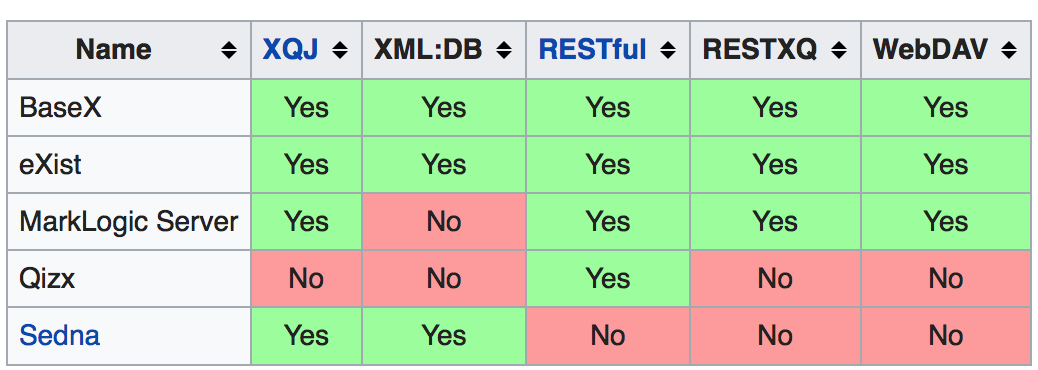
\includegraphics[width=\textwidth]{figures/XML_apis.png}
\end{column}
\end{columns}

\vskip1em

Unlike with relational data, however, XML systems must also expose them as documents which can be opened, edited, and saved by XML (file) editors. 

\end{frame}

\begin{frame}[fragile]{XQJ: XQuery API for Java}

XQJ was developed by the Java community and backed by major vendors (including Oracle and IBM); it became a standard in 2009. 

\bgroup
\lstset{
	language=Java,
	basicstyle=\ttfamily\scriptsize,
	commentstyle=\color{fern},
	stringstyle=\color{stringColor},
	keywordstyle=\sffamily\color{functionColor},
	emphstyle=[1]\color{datatypeColor},
	emph=[1]{conn,expr,result},
	emphstyle=[2]\color{blue},
	emph=[2]{getItemAsString,XQExpression,XQConnection,createExpression,close}
}

\begin{lstlisting}
// Create a new connection to an XML database
XQConnection conn = vendorDataSource.getConnection("myUser", "myPassword");

XQExpression expr = conn.createExpression(); // reusable XQuery Expression

XQResultSequence result = expr.executeQuery(
  "for $n in fn:collection('catalog')//item " +
  "return fn:data($n/name)"); // execute an XQuery expression

// Process the result sequence iteratively
while (result.next()) {
  // Print the current item in the sequence
  System.out.println("Product name: " + result.getItemAsString(null));
}

// Free all resources created by the connection
conn.close();
\end{lstlisting}
\egroup

\end{frame}

\begin{frame}[fragile]{Parameterized XQuery}

As with SQL, programs can pass parameters to an XQuery processor at runtime, via \textbf{external variables} in the query.

\bgroup
\lstset{
	language=Java,
	basicstyle=\ttfamily\scriptsize,
	commentstyle=\color{fern},
	stringstyle=\color{stringColor},
	keywordstyle=\sffamily\color{functionColor},
	emphstyle=[1]\color{datatypeColor},
	emph=[1]{conn,expr,result},
	emphstyle=[2]\color{blue},
	emph=[2]{getItemAsString,XQExpression,XQConnection,createExpression,close},
	moredelim = [is][\color{purple}\ttfamily]{-:}{:-}
}

\begin{lstlisting}
XQExpression expr = conn.createExpression();

// The XQuery expression to be executed
String es = -:"declare variable $x as xs:integer external;":- +
            " for $n in fn:collection('catalog')//item" +
            " where $n/price <= $x" +
            " return fn:data($n/name)";

// Bind a value (21) to an external variable with the QName x
expr.bindInt(new QName("x"), 21, null);

// Execute the XQuery expression
XQResultSequence result = expr.executeQuery(es);

while (result.next()) {
  // Process the result ...
}
\end{lstlisting}
\egroup
\end{frame}

\begin{frame}{XQJ Adoption}

Although not the only XQuery API out there, XQJ\footnote{\url{https://en.wikipedia.org/wiki/XQuery_API_for_Java}} is well supported.

\begin{itemize}[-]
\item \alert{File-based XQuery Processors}: Saxon XSLT and XQuery processor, \textcolor{blue}{Zorba}, MXQuery, Oracle XQuery Processor.

\item \alert{Native Systems}: MarkLogic, eXist, BaseX, Sedna, Oracle XDB, Tamino, TigerLogic, ...

\item \alert{Relational Systems}: Oracle DB (Not XDB), IBM DB2, Microsoft SQL Server, Sybase ASE, Informix, \textcolor{gray}{MySQL}, \textcolor{blue}{PostgreSQL}
\end{itemize}

Supporting= relational systems is not easy, because each implements XML in a different way. 
\end{frame}

\begin{frame}{ACID Transactions with XQJ}

From their manual (coloring added):

\vskip1em

\begin{quote}
By default a connection operates in auto-commit mode, which means that \alert{each XQuery is executed and committed in an individual transaction}. If auto-commit mode is disabled, a transaction must be ended explicitly by the application calling commit() or rollback().

An XQConnection object can be created on top of an existing JDBC connection. If an XQConnection is created on top of the JDBC connection, it inherits the transaction context from the JDBC connection.
\end{quote}

\end{frame}
















\end{document}